
%% Template by Michal Forisek


\documentclass[a4paper]{report}
\usepackage{slovak}
\usepackage[utf8]{inputenc}
\usepackage{a4wide}
\usepackage{tabularx}
\usepackage{amsfonts}
\usepackage{amssymb}
\usepackage{amsmath}
\usepackage{epsfig}
\usepackage{color}
\usepackage{mathrsfs}
\usepackage{verbatim}
\usepackage{hyperref}
\usepackage{algorithm2e}

% vim: set fdm=marker:
%% Original by Michal Forisek

\ifx \RestyleAlgo \undefined
    \def\RestyleAlgo#1{\restylealgo{#1}}
\fi

\RestyleAlgo{boxed} %% nastav styl algorithm2e

%% zakladne definicie
\newcommand{\quoteme}[1]{\clqq#1\crqq}
\def\todo#1{[{\color{red} TODO:} {\bf  #1}]}
\def\fixme#1{[{\color{red} FIXME:} {\bf  #1}]}
\def\verify#1{\todo{verify: #1}}

\def\xor{\oplus}
\def\concat{\|}
%\def\inr{\in_{R}}
\def\toa #1 {\overset{#1}{\rightarrow}}
\def\inr{\overset{\$}{\leftarrow}}
\def\assign{\leftarrow}
\def\send{\rightarrow}
\def\isomorph{\cong}
\def\nsd{NSD}
\def\union{\cup}
\newcommand{\unit}[1]{\ensuremath{\, \mathrm{#1}}}
\DeclareMathOperator{\dlog}{dlog}

\def\compactlist{
  \setlength{\itemsep}{1pt}
  \setlength{\parskip}{0pt}
  \setlength{\parsep}{0pt}
}
\def\mod{\,{\rm mod}\,}

%%% original od Misofa:
%% {{{

\catcode`\@=11

\def\R{{\cal R}}
\def\cent{{c\kern-0.3em|\kern0.1em}}
\def\N{{N}} % FIXME FIXME 

\let\eps=\varepsilon

\def\relupdown#1#2#3{\mathrel{\mathop{#1}\limits^{#2}_{#3}} }

\let\then=\Rightarrow
\let\neht=\Leftarrow

\def\krok#1{\relupdown{\Longrightarrow}{}{#1}}
\def\thenrm{\relupdown{\Longrightarrow}{}{rm}}

\def\bicik{\upharpoonright}
\def\B{{\mathbf B}}
\def\kodTS#1{{\tt <}#1{\tt >}}

\newtheorem{definicia}{Definícia}[section]
\newtheorem{HLPpoznamka}{Poznámka}[section]
\newtheorem{HLPpriklad}{Príklad}[section]
\newtheorem{HLPcvicenie}[HLPpriklad]{Cvičenie}
\newtheorem{zadanie}{Úloha}[section]
\newenvironment{poznamka}{\begin{HLPpoznamka}\rm}{\end{HLPpoznamka}}
\newenvironment{priklad}{\begin{HLPpriklad}\rm}{\end{HLPpriklad}}
\newenvironment{cvicenie}{\begin{HLPcvicenie}\rm}{\end{HLPcvicenie}}
\newtheorem{veta}{Veta}[section]
\newtheorem{lema}[veta]{Lema}
\newtheorem{dosledok}[veta]{Dôsledok}
\newtheorem{teza}[veta]{Téza}
% \newtheorem{dokaz}{Dôkaz}[section]

\long\def\odsadene#1{
\leftskip=\parindent
\parindent=0pt
\vskip-5pt

\parskip=5pt
#1
\parskip=0pt

\parindent=\leftskip
\leftskip=0pt

} % end \odsadene




%%%%%%%%%%% PROSTREDIE PRE PISANIE KOMENTAROV

%\newenvironment{komentar}{%
%\vskip\baselineskip
%\tabularx{0.95\textwidth}{|X|}
%\sl
%}
%{\endtabularx
%\vskip\baselineskip
%}

\newenvironment{komentar}{%
\vskip\baselineskip\noindent
\tabularx{\textwidth}{>{\hsize=.2\hsize}X>{\hsize=1.8\hsize}X}
\sl ~ & \sl
}
{\endtabularx
\vskip\baselineskip
}

%\newenvironment{komentar}{%
%\vskip\baselineskip
%\trivlist\vspace{-4pt}\raggedleft\item\relax\tabularx{0.9\textwidth}{X}\sl}
%{\endtabularx\vspace{-4pt}\endtrivlist
%\vskip\baselineskip
%}

\newenvironment{dokaz}{\trivlist
  \item[\hskip \labelsep{\bfseries Dôkaz.}]}{\endtrivlist}
  
%\newenvironment{dokaz}{%
%\vskip\baselineskip\noindent
%\tabularx{\textwidth}{||X||}
%\sl
%}
%{\endtabularx
%\vskip\baselineskip
%}

%%%%%%%%%%% PROSTREDIE PRE MOJE ITEMIZE 

\newenvironment{myitemize}{%
\begin{itemize}
\itemsep-3pt
}
{\end{itemize}
}

%%%%%%%%%%% MATICKE MAKRA

\font\tenrm=csr10

\def\eps{\varepsilon}
% \def\R{{\mathbb R}}
\def\lvec#1{\overrightarrow{#1}}
\def\uhol{{\measuredangle}}
\def\then{\Rightarrow}
% \def\lg{{\rm lg}}
\def\lg{\log_2}
%\def\div{\mathbin{\rm div}}
\def\div{{\rm div}}

%%%%%%%%%%% PDF

\newif\ifpdf
\ifx\pdfoutput\undefined
  \pdffalse
\else
  \pdfoutput=1 \pdftrue
\fi

%%%%%%%%%%% OBRAZKY 

\newcommand{\myincludegraphics}[2][]{\includegraphics[#1]{images/#2}}

%%%%%%%%%%% SLOVNICEK

\openout2=\jobname.slo

\newcommand{\definuj}[3][]{%
\def\tmpvoid{}\def\tmpfirst{#1}%
\ifx\tmpvoid\tmpfirst%
  {\sl #2}\label{definicia:#2}\write2{#2 & #3 & \pageref{definicia:#2} \cr}%
\else%
  {\sl #2}\label{definicia:#2}\write2{#1 & #3 & \pageref{definicia:#2} \cr}%
\fi}

\newcommand{\definujsilent}[2]{%
\label{definicia:#1}\write2{#1 & #2 & \pageref{definicia:#1} \cr}%
}

\newcommand\myglossary{
  \immediate\closeout2 
  %\if@twocolumn\@restonecoltrue\onecolumn\else\@restonecolfalse\fi
  \chapter{Slovníček pojmov}
  \begin{tabular}{|l|l|r|}
  \hline
  {\bfseries slovenský pojem} & {\bfseries anglický preklad} & {\bfseries str.} \\ 
  \hline
  \InputIfFileExists{\jobname.srs}{}{~ & ~ & ~ \\}
  \hline
  \end{tabular}
  %\if@restonecol\twocolumn\fi
}

%%%%%%%%%%% UVODZOVKY

\catcode`\"=13
\def "{\begingroup\clqq\def "{\endgroup\crqq}}
\def\dospecials{\do\ \do\\\do\{\do\}\do\$\do\&%
  \do\#\do\^\do\^^K\do\_\do\^^A\do\%\do\~\do\"}

%%%%%%%%%%% DANGER BENDS 

\font\manual=manfnt % font used for the METAFONT logo, etc.
\def\dbend{{\manual\char127}} % dangerous bend sign

\newlength{\bendwidth}   \settowidth{\bendwidth}{\dbend}    \newlength{\hangwidth}

\def\hangone{%
  \hangwidth=\bendwidth%
  \advance\hangwidth 5pt%
  \hangindent\hangwidth%
}
\def\hangtwo{%
  \hangwidth=\bendwidth%
  \multiply\hangwidth 2%
  \advance\hangwidth 6pt% 
  \hangindent\hangwidth%
}

\def\medbreak{\par\ifdim\lastskip<\medskipamount \removelastskip\penalty-100\medskip\fi}
\let\endgraf=\par

\def\d@nger{\medbreak\begingroup\clubpenalty=10000
%\def\d@nger{\begingroup\clubpenalty=10000
%  \def\par{\endgraf\endgroup\medbreak} \noindent\hangone\hangafter=-2
  \def\par{\endgraf\endgroup} \noindent\hangone\hangafter=-2
  \hbox to0pt{\hskip-\hangindent\dbend\hfill}}
\outer\def\danger{\d@nger}

\def\dd@nger{\medbreak\begingroup\clubpenalty=10000
%  \def\par{\endgraf\endgroup\medbreak} \noindent\hangtwo\hangafter=-2
  \def\par{\endgraf\endgroup} \noindent\hangtwo\hangafter=-2
  \hbox to0pt{\hskip-\hangindent\dbend\kern1pt\dbend\hfill}}
\outer\def\ddanger{\dd@nger}

\def\enddanger{\endgraf\endgroup} % omits the \medbreak
\def\enddangerhop{\endgraf\endgroup\medbreak}




\def\@nakedcite#1#2{{#1\if@tempswa , #2\fi}}
\DeclareRobustCommand\nakedcite{%
  \@ifnextchar [{\@tempswatrue\@nakedcitex}{\@tempswafalse\@nakedcitex[]}}
\def\@nakedcitex[#1]#2{%
  \let\@citea\@empty
  \@nakedcite{\@for\@citeb:=#2\do
    {\@citea\def\@citea{,\penalty\@m\ }%
     \edef\@citeb{\expandafter\@firstofone\@citeb\@empty}%
     \if@filesw\immediate\write\@auxout{\string\citation{\@citeb}}\fi
     \@ifundefined{b@\@citeb}{\mbox{\reset@font\bfseries ?}%
       \G@refundefinedtrue
       \@latex@warning
         {Citation `\@citeb' on page \thepage \space undefined}}%
       {\hbox{\csname b@\@citeb\endcsname}} }}{#1}}

\long\def\FIXME#1{
  \begin{center}
  \begin{minipage}{0.8\textwidth}
  {\bf FIXME:~}\sl #1
  \end{minipage}
  \end{center}
}


\catcode`\@=12
%% }}}


\begin{document}

\thispagestyle{empty}
\begin{minipage}{0.25\textwidth}

\includegraphics[width=0.9\textwidth]{img/komlogo-new}
\end{minipage}
\begin{minipage}{0.69\textwidth}
\begin{center}
\sc Katedra Informatiky \\
Fakulta Matematiky, Fyziky a Informatiky \\
Univerzita Komenského, Bratislava
\end{center}
\end{minipage}

\vfill
\begin{center}
\begin{minipage}{0.8\textwidth}
\hrule
\bigskip\bigskip
\centerline{\LARGE\sc Krypto II}
\smallskip
\centerline{(spísané poznámky, draft)}
\bigskip
\bigskip
\centerline{\large\sc Vladimír Boža, Peter Perešíni}
\bigskip
\centerline{\large\sc (prednášal RNDr. Martin Stanek, PhD.)}
\bigskip\bigskip
\hrule
\end{minipage}
\end{center}
\vfill
{~}
\hfill verzia zo dňa {\bf\today} 
\eject % EOP i

\section*{Úvod a disclaimer}

Tieto poznámky obsahujú študijné materiály k predmetu 
\emph{Kryptológia II}
na Fakulte matematiky, fyziky a informatiky UK.
Základná verzia bola spísaná podľa prednášky RNDr. Martina Staneka v
roku 2010. Poznámky však nie sú oficiálny študijný materiál, preto
autori neručia za ich aktuálnosť a vhodnosť na štúdium. Navyše, obsah
prednášky sa môže z roka na rok meniť, a preto je odporúčané dávať
pozor na prípadné rozdiely a dopísať si časti nepokryté týmito
poznámkami.

Aby sme umožnoli jednoduchšie spravovanie a udržali poznámky dlhšie
aktuálne, rozhodli sme sa verejne publikovať zdrojové kódy na stránke
\url{http://code.google.com/p/krypto2}. Ak máte akékoľvek pripomienky,
návrhy, opravy, môžete nám ich prostredníctvom tejto stránky oznámiť.

PPershing a U\$ama.


\tableofcontents

\chapter{Úvod}
\label{chapter:uvod}
\section{Prerekvizity a označenia}

\todo{odkaz na skripta z krypto I}

V zvyšnom texte budeme dodržiavať (až na občasné výnimky) nasledujúce
označenia:
\begin{itemize}
\item $A,B$ - účastníci komunikácie, $E$ - útočník, $E(A)$ - útočník
            tváriaci sa ako účastník $A$.
\item $E(p,k); E_k(p)$ - zašifrovanie otvoreného textu $p$ pomocou kľúča $k$
\item $D(c,k); D_k(c)$ - odšifrovanie šifrového textu $c$ pomocou kľúča $k$
\item $E_A(m)$ - zašifrovanie správy $m$ pomocou verejného kľúča účastníka $A$
\item $D_A(c)$ - odšifrovanie správy $c$ pomocou súkromného kľúča účastníka $A$
\item $H(t)$ - spracovanie textu $t$ pomocou hashovacej funkcie $H$
\item $x \inr M$ - $x$ je \emph{náhodne zvolený} prvok množiny $M$
\item $\exists !$ - existuje práve jeden
\item $p(A)$ - pravdepodobnosť javu $A$
\item $p(A|B)$ - podmienená pravdepodobnosť, čiže aká je pravdepodobnosť javu $A$, ak platí $B$
\end{itemize}

\section{Prerekvizity}

\section{Označenia}

\begin{itemize}
\item $E(p,k); E_k(p)$ - zašifrovanie otvoreného textu $p$ pomocou kľúča $k$
\item $D(c,k); D_k(c)$ - odšifrovanie šifrového textu $c$ pomocou kľúča $k$
\item $E_A(m)$ - zašifrovanie správy $m$ pomocou verejného kľúča účastníka $A$
\item $D_A(c)$ - odšifrovanie správy $c$ pomocou súkromného kľúča účastníka $A$
\item $H(t)$ - spracovanie textu $t$ pomocou hashovacej funkcie $H$
\end{itemize}

\section{0. prednáška (Ako (ne)šifrovať disky}

V decembri 2009 bola nájdená bezpečnostná chyba v niektorých šifrovaných USB diskoch
(Kingston DataTraveler BlackBox, SanDisk Cruzer Enterprise FIPS Edition a
Verbatim Corporate Secure FIPS Edition). Všetky výrobcovia uvádzajú, že disky
spĺňajú bezpečnostný štandart FIPS 140-2 a používajú úplne rovnaký systém zabezpečenia,
ktorý vyzerá nasledovne:
\begin{itemize}
\item Používateľ zadá disku heslo.
\item Heslo za pretransformuje cez MD5 hash a prvá polovica výslednej hashe sa použije ako kľúč K.
\item Následne sa pomocou AES-256 a kľúča K odšifruje daných 32 bajtov z disku (označme ich $X$). Potom zistí, či
$D_K(X)=C$, kde $C$ je pevne známa konštanta (u všetkých výrobcov dokonca rovnaká). Ak áno, tak sa disk odomkne a dáta sa sprístupnia.
Ak nie, tak sa požiadavka zamietne. Dešifrovanie ostatných dát nezávisí od hesla.
\end{itemize}

\begin{figure}[htp]
    \centering
    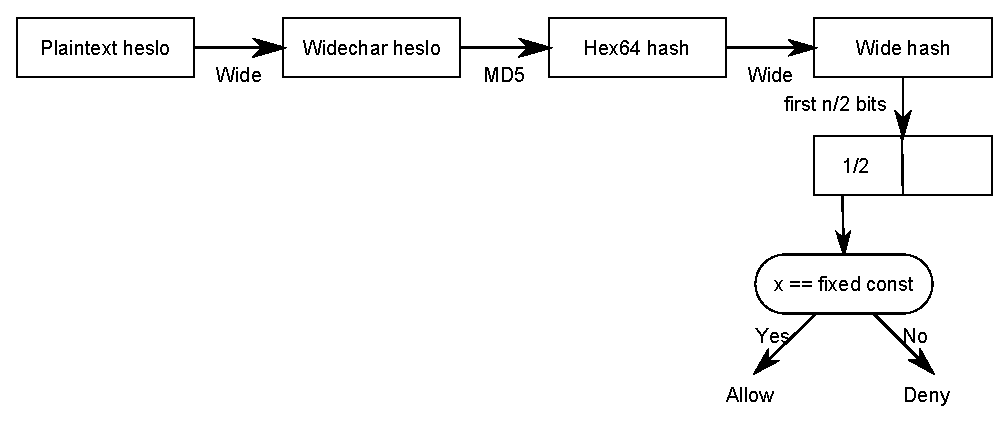
\includegraphics[scale=0.75]{img/0/extern_drive_encryption}
    \label{fig:extern_drive_encryption}
    \caption{Šifrovanie externého disku}
\end{figure}

Útok na tento systém je vcelku jednoduchý. Stačí v pamäti prepísať výsledok dešifrovacej transformácie. 

%Viac na:
%\url{http://www.h-online.com/security/news/item/NIST-certified-USB-Flash-drives-with-hardware-encryption-cracked-895308.html}

%A ešte na (pekny dokument nie priamo suvisiaci):
%Investigating 'secure'USB stickspsu.edu [PDF]
%PJ Bakker… - Citeseer
%\url{http://citeseerx.ist.psu.edu/viewdoc/download?doi=10.1.1.84.2539&rep=rep1&type=pdf}



\chapter{Krypto I}
\label{chapter:krypto}
\section{Interaktívne dokazovacie systémy}

V tejto časti sa budeme venovať dokazovacím systémom. Pôjde o akýsi
typ spoločného výpočtu dvoch účastníkov - jedného výpočtovo
neobmedzeného provera $P$ a výpočtovo obmedzeného overovateľa $V$.
Cieľom provera je akýmsi spôsobom presvedčiť overovateľa o znalosti
nejakého faktu.
Formálne,
interaktívnym dokazovacím systémom nazveme dvojicu
$\langle P,V \rangle$, kde $P$ je pravdepodobnostný TS s neobmedzenou výpočtovou silou,
$V$ je pravdepodobnostný TS pracujúci v polynomiálnom čase.
Oba stroje zdieľajú spoločný vstup $x$, môžu počas svojho výpočtu
komunikovať a o akceprovaní resp. zamietaní vstupu $x$ rozhoduje iba
$V$.
IDS pre jazyk $L$ je $\langle P,V \rangle$ pre ktorý platí
\begin{itemize}
\item {\bf úplnosť} - $\forall x \in L: 
    Pr[V\textit{ akceptuje } x \textit{ v systéme } 
        \langle P,V \rangle ] \ge 2/3$
\item {\bf korektnosť} - $\forall P^*: \forall x \not \in L: 
    Pr[V\textit{ akceptuje } x \textit{ v systéme } 
        \langle P^*,V \rangle ] \le 1/3$
\end{itemize}
Prvá podmienka hovorí o tom, že ak $x\in L$, dokazovateľ s veľkou
pravdepodobnosťou presvedčí overovateľa o správnosti.
Naopak, korektnosť tvrdí, že ľubovoľný (podvodný) dokazovateľ
presvedčí overovateľa na zlom vstupe len s nízkou pravdepodobnosťou.

\begin{komentar}
    Pre $L \in P$ je jednoduché navrhnúť IDS. Overovateľ bude ignorovať
    komunikáciu a môže si vypočítať príslušnosť slova sám.
    Pre $L \in NP$ je jednoduché navrhnúť IDS posielajúci práve jednu
    správu - konkrétny dôkaz - výpočet NTS pre problém L.
\end{komentar}

\begin{priklad}
    Uvažujme problém $GNI \not \in NP$ - grafový neizomorfizmus.
    Vstup pozostáva zo zápisu dvoch grafov $G_0, G_1$, akceptovať chceme, keď
    dané dva grafy nie sú izomorfné. Môžeme použiť nasledovný protokol
    pri dôkaze: Uvažujme $k$ kôl, v každom z nich prebehne nasledujúca
    komunikácia:
    \begin{itemize}
        \item $V$ si zvolí $i \inr \{0,1\}$, permutáciu
         $\pi \inr perm(|G_0|)$
        \item $P \send V: H = \pi(G_i)$.
        \item $V \send P: i'$ reprezentujúce graf $G$, s ktorým je $H$
        izomorfný. ($V$ je neobedzene výpočtovo silný)
        \item prover zamietne ak $i \not = i'$.
    \end{itemize}
    Po $k$ úspešných kolách $V$ akceptuje.

    Ak $G_0 \isomorph G_1$, tak $P$ má v každom kole šancu 50\% na
    uhádnutie indexu $i$, ktorý si vymyslí $V$. 
    Pravdepodobnosť akceptovania po $k$ kolách je teda $2^{-k}$.
    Naopak, ak $G_0 \not \isomorph G_1$, tak čestný dokazovateľ vie
    vždy odlíšiť $G_0$ od $G_1$ a teda akceptujeme s pravdepodobnosťou 1.
\end{priklad}

\todo{dosiahnute vysledky}:
IP = QIP (Quantum Interactive proof) = PSPACE
MIP = NEXPTIME
\todo{pridat referencie na clanky}


\section{Zero knowledge}
Špeciálnym prípadom interaktívnych dokazovacích systémov sú takzvané
bezznalostné dôkazy. Základná myšlienka sa dá ilustrovať na príklade 
"Alibaba a jaskyňa tajomstiev".

Alibaba na svojich potulkách narazil (alebo skôr naďabil) na jaskyňu,
ktorá sa na vyslovenie čarovnej formuly otvorí. Po dlhšom skúmaní
prišiel na to, že jazkyňa vyzerá ako na obr. \ref{fig:alibaba}. Pretože v
jaskyni neboli žiadne poklady (alebo boli, ale niekto ich stihol
vybrať skorej), Alibaba sa rozhodol zbohatnúť na TV show.
Bude ukazovať, že vie tajnú formulku a nafilmujú ho pritom. Nechce ale
prezradiť tajomstvo zvyšku sveta.

\begin{figure}[htp]
    \centering
    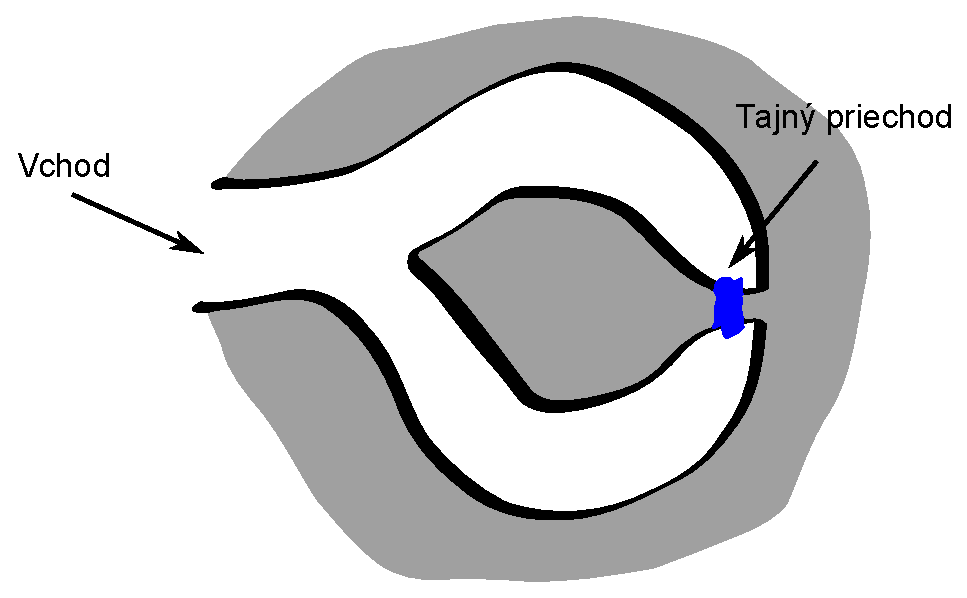
\includegraphics[scale=0.4]{img/x/alibaba}
    
    \label{fig:alibaba}
    \caption{Alibabova jaskyňa}
\end{figure}

Preto sa s filmármi dohodol na nasledujúcom postupe - vôjde do jaskyne
sám. Následne dnu vojde aj filmový štáb a ten zakričí Aladinovi, z
ktorej strany má dôjsť. Ten na demonštráciu znalosti prechádzania cez
steny vyjde zo správnej strany.

Poučenie z príbehu: Môžeme si všimnúť, že Aladin nikomu neprezradí
svoje tajomstvo. Zároveň ale presvedčí štáb o tom, že cez tie steny
chodí, pretože inak by si musel vedieť niekoľkokrát po sebe správne
tipnúť, čo sa mu rozhodnú zakričať, keď dôjdu na rázcestie.
Dôkaz má ale aj ďalšiu vlastnosť - Aladin síce presvedčil štáb, ale
môže presvedčiť aj divákov? Nie. Čo ak bolo napríklad video
"nastrihané" iba na dobré pokusy?

Bezznalostné dokazovacie systémy sú preto také systémy, pri ktorých
dokazovateľ presvedčí overovateľa o svojej pravde bez toho aby mu
prezradil čokoľvek iné. Taktiež, ľubovoľný externý pozorovateľ
komunikácie nemá byť schopný odlíšiť reálny dôkaz od akéhosi
vykonštruovaného.


\todo{zvysok, blackbox simulator}
\todo{ZK pre izomorfizmus}
\todo{preco neizomorfixmus (ako je prezentovany) nie je ZK}

\section{Bit commitment}

Bit commitment schéma je protokol pre dvoch účastníkov, kde sa najprv účastník
zaviaže k nejakému bitu (ktorý zatiaľ zostáva utajený pre ostatných) 
a následne po istom čase ho odhalí. Formálne to môžeme definovať takto:

\begin{definicia}
Majme dve množiny $X,Y$ a funkciu $f\colon \{0,1\} \times X \to Y$, ktorú vieme
\clqq ľahko\crqq počítať. Od $f$ požadujeme navyše ešte tieto vlastnosti:
\begin{itemize}
\item Zo znalosti $f(b,x)$ je ťažké určiť $b$ - vlastnosť utajenia.
\item Je ťažké nájsť $x, y$ také, že $x \neq y$ a $f(0,x) = f(1,y)$ - vlastnosť záväznosti.
\end{itemize}
Potom bit commitment protokol vyzerá nasledovne:
\begin{enumerate}
\item $A$ zvolí $b \in \{0,1\}$ ku ktorému sa chce zaviazať a $x \inr X$
\item $A \to B$: $y = f(b,x)$ - záväzok
\item $A \to B$: $x$ - odhalenie, môže prísť po istom čase
\item $B$ overí, či $y = f(0,x)$ alebo $y = f(1,x)$
\end{enumerate}
\end{definicia}

Tento protokol môžeme realizovať viacerými spôsobmi. 

\subsection{Bit commitment pomocou RSA}

Majme nejakú inštanciu RSA systému, teda trojicu $(n,e,d)$, kde účastník $b$ nepozná súkromný kľúč.
Bit commitment realizujeme nasledovne:
\begin{enumerate}
\item Záväzok: $A$ si zvolí $x \inr \mathbb{Z}_n^*$ a pošle $B$: $y = x^e \pmod n$, v tomto prípade je $b$ najmenej signifikatný bit z $x$
\item Odhalenie: $A$ pošle $x$. $B$ overí, či $x^e \pmod n = y$
\end{enumerate}

Vlastnosť utajenia je dodržaná, keďže možnosť zistiť $b$ je ekvivalentná rozbitiu RSA schémy.
Vlastnosť záväznosti je tiež dodržaná, keďže k jednému $y$ existuje iba jedno $x$. V tomto prípade ide o nepodmienenú bezpečnosť.

\subsection{Bit commitment pomocou diskrétneho logaritmu}
Majme konečnú grupu $G$ a $g, h \in G$, pričom v tejto grupe nevieme efektívne rátať diskrétny logaritmus. Zároveň
nevieme diskrétny logaritmus $h$ pri základe $g$.  Realizácia funkcie $f(b,x)$ bude nasledovná: $$f(b,x) = g^x h^b$$

Utajenie je v tomto prípade nepodmienene bezpečné, lebo existujú $x, y$ také, že: $g^x = g^y h$ a teda nevieme jednoznačne
určiť $b$ zo znalosti $f(b,x)$.
Vlastnosť záväznosti výplýva z toho, že nepoznáme diskrétny logaritmus $h$ pri základe $g$.

Môžeme si všimnúť, že sme vedeli dosiahnúť pri jednej vlastnosti (utajenie, záväznosť) nepodmienenú bezpečnosť.
Nasledujúca veta hovorí o tom, že nepodmienenú bezpečnosť nevieme dosiahnúť pri oboch vlastnostiach.

\begin{veta}
Neexistuje bit commitment schéma, ktorá by garantovala nepodmienenú bezpečnosť pri utajení a záväznosti.
\end{veta}

\begin{dokaz}
Sporom. 
Uvažujeme funkciu bit commitment schémy $f(b,x)$. Ak je táto schéma garantuje nepodmienenú záväznosť, tak
platí $\forall x, y\colon f(x,b_1) = f(y,b_2) \Rightarrow b_1 = b_2$ (teda neexistuje vhodná dvojica
$x, y$ ktorou by sme vedeli porušiť záväzok). Z toho vyplýva, že keď dostaneme $z = f(x,b)$, tak vieme 
vyskúšaním všetkych $(x,b)$ určiť vyhovujúcu dvojice, ktoré ale budú mať rovnaký commitnutý bit.
A teda táto schéma nemôže garantovať nepodmienené utajenie.
\end{dokaz}
\todo{IDS pre ham cycle pomocou BC}



\section{Oblivious transfer}

Ďalším základným primitívom, na ktorom vieme budovat kryptografické
prvky je takzvaný oblivious transfer. Ide o akýsi prenos údajov,
pričom sender sa nedozvie, či boli údaje prenesené, prípadne ktoré
údaje boli prenesené.

\begin{definicia}[1-2 OT]
    1-2 oblivious transferom nazveme komunikáciu podľa nasledujúcej
    schémy:
    \begin{itemize}
        \item $A \send B: m_0, m_1$, kde $m_0$ a $m_1$ sú 2 rôzne
        správy, ktoré chce $A$ poslať.
        \item $B$ si vyberie niektorú zo správ, ktorú chce prijať a
        toto prijatie mu bude umožnené.
        \item $A$ sa nedozvie, ktorú správu $B$ prijal.
        \item $B$ nemá možnosť prijať obe správy naraz.        
    \end{itemize}
\end{definicia}

\begin{definicia}[50\% OT]
    50\% oblivious transferom nazveme komunikáciu podľa nasledujúcej
    schémy:
    \begin{itemize}
        \item $A \send B: m$, kde $m$ je správa.
        \item $B$ s spravdepodobnosťou 50\% správu prijme, inak sa o
        nej nedozvie nič.
        \item $A$ sa nedozvie, či $B$ správu prijal
    \end{itemize}
\end{definicia}

\begin{priklad}[Realizácia 50\% OT]
    Nech $A$ chce poslať správu účastníkovi $B$ s 50\%-nou
    pravdepodobnosťou úspechu. Na začiatku si $A$ zvolí inštanciu RSA
    s $n=pq$, kde $p,q$ sú veľké prvočísla. Bude nasledovať
    komunikácia
 \begin{itemize}
    \compactlist
    \item $A \send B: n,e,E(m)$ 
    \item $B$ si zvolí $x \inr Z_n$
    \item $B \send A: x^2$
    \item $A$ s pomocou faktorizácie vyberie nejakú odmocninu
        $z \inr \{x,-x,y,-y\}$.
    \item $A \send B: z$.
    $B$ vie faktorizovať $n$ (a dešifrovať správu) s
    pravdepodobnosťou 50\% (ak $z \not = \pm x$, tak jednoducho
    spočíta pomocou $\nsd(z-x, n)$).
 \end{itemize} 
\end{priklad}

\begin{priklad}[Realizácia 1-2 OT]
 1-2 OT budeme realizovať za pomoci diskrétneho logaritmu.
 Účastník $A$ si zvolí grupu $G$, $n=|G|$ a generátor $g\in G$.
 \begin{itemize}
    \compactlist
    \item $A \send B: c \inr G$.
    \item $B$ si zvolí $b\in\{0,1\}$ - číslo správy, ktorú chce
    prijať.
    \item $B$ si zvolí $x \inr G$ a vypočíta hodnoty $y_b = g^x$,
    $y_{1-b} = c/ y_b$. Platí $y_0 y_1 = c$ a tiež existuje (pretože
    $g$ je generátor) hodnota $x': g^{x'} = y_{1-b}$. Teda, $A$ nevie
    odlíšiť jednotlivé hodnoty.
    \item $B \send A: y_0$.
    \item $A$ si zvolí $k_0,k_1 \inr G$ a vytvorí šifrované správy 
    $E_0 = \langle g^{k_0}, y_0^{k_0} \xor m_0 \rangle$,
    $E_1 = \langle g^{k_1}, y_1^{k_1} \xor m_1 \rangle$.
    \item $A \send B: E_0, E_1$.
    \item $B$ dešifruje $m_b$ ako $(g^{k_b})^x \xor (y_b ^ {k_b} \xor
    m_b)$.
    Pokiaľ $B$ nevie riešiť DH problém, druhú správu nedostane.
    \todo{dokaz}
 \end{itemize}
\end{priklad}

\subsection{Konverzie}

\begin{lema}
    50\% OT sa dá simulovať pomocou 1-2 OT.
\end{lema}
\begin{dokaz}
    Postup je jednoduchý. Nech $A$ chce poslať správu 
    $m \ne 0$.\footnote{Predpokladáme, že vieme posielať správy, ktoré
        sú dlhšie ako 1 bit.\fixme{ako spravit konveziu z 1 bitu?}
    }
    Nech $c \inr \{0,1\}$ a nech $m_c = m, m_{1-c} = 0$. $A$ pošle
    správy $m_0, m_1$ pomocou 1-2 OT. $B$ prijme správu $m$ s
    pravdepodobnosťou 50\%, inak prijme 0 a vie, že sa prenos
    nepodaril.
\end{dokaz}

\todo{1-2 OT pomocou 50}
\todo{BC pomocou 50 OT}
Pre záujemcov je predchádzajúca konštrukcia presnejšie popísaná v
\cite{ot_equiv}.

\section{Bezpecny vypocet viacerych ucastnikov}

\todo{porovnavanie veku}
\todo{\url{http://www.derkeiler.com/Newsgroups/sci.crypt/2006-10/msg00665.html}}

\todo{bezpecny vypocet funkcie}



\chapter{Krypto II}
\label{chapter:krypto2}
\section{Absolútne bezpečná šifra}

Tento krát sa ideme zaoberať nepodmienenou bezpečnosťou. Uvažujme 
výpočtovo neobmedzene silného útočníka a cypher text only attack (COA).
Požadujeme aby útočník zo znalosti šifrového textu nezískal nič nové.

Označme množinu otvorených textov ako $P$, kľúčov ako $K$, šifrových textov ako $C$
(uvažujeme iba množinu reálne možných šifrových textov). Každému $x \in P$ vieme priradiť
pravdepodobnosť výskytu $pr(x)$, pravdepodobnosť
výskytu konkrétneho kľúča $k \in K$ označíme ako $pr(k)$. Predpokladáme, že
konkrétny kľúc používame iba raz a že jeho voľba nezávisí od otvoreného textu.
Takisto pravdepodobnosť výskytu šifrového textu $c \in C$ označíme $pr(c)$. Táto pravdepodobnosť
bude vždy väčšia ako nula (keďže uvažujeme len šifrové texty, ktoré môžu vzniknúť zašifrovaním).
Všetky tieto množiny považujeme za konečné.

\begin{definicia}
    Šifrovací systém $(E,D)$ je absolútne bezpečný ak:
    $$\forall x \in P, \forall c \in C\colon pr(x | c) = pr(x)$$
\end{definicia}
\begin{komentar}
    Táto definícia vlastne hovorí o tom, že znalosť šifrového textu útočníkovi nepovie nič
    nové, keďže distribúciu pravdepodobnosti otvorených textov pozná.
\end{komentar}

Niekoľko zaujímavých vlastností:
Vzhľadom na to, že dešifrovanie musí byť uskutočniteľné, musí platiť $|C| \geq |P|$.
Ďalej určite platí $|K| \geq |P|$, ináč by sme pri znalosti šifrového textu mohli 
vyskúšať dešifrovanie všetkými kľúčmi a niektoré otvorené texty by sme mohli vylúčiť
($pr(x|c) = 0$). Zaujímavá je situácia keď $|P| = |C| = |K|$, tú popisuje nasledujúca veta:

\begin{veta}{(Shanon)}
    Nech $(E,D)$ je šifrovací systém, kde $|P|=|C|=|K|$. Potom tento šifrovací systém je
    absolútne bezpečný práve vtedy, keď sú splnené nasledujúce vlastnosti:
    \begin{enumerate}
        \item $\forall k \in K\colon pr(k) = \frac{1}{|K|}$
        \item $\forall x \in P, \forall y \in C: \exists! k \in K\colon E_k(x) = y$
    \end{enumerate}
\end{veta}

\begin{dokaz}
    \noindent
    \begin{itemize}
    \item[$\Rightarrow:$] 
        Nech systém $(E,D)$ je absolútne bezpečný.
        Ak by pre $x \in P, y \in C$ neexistoval kľúč $k \in K$ taký, 
        že $E_k(x) = y$, útočník zo znalosti $y$ vie vylúčiť otvorený text $x$,
        čo odporuje tomu, že systém $(E,D)$ je absolútne bezpečný. 
        Keďže $|C|=|K|$, tak tento kľúč môže byť maximálne jeden 
        (keby ich bolo viac, tak by $\exists z \in C$ taký, že
        $x$ nevieme zašifrovať na $z$). 

        Keďže $P$ je konečná, môžeme otvorené texty očíslovať, 
        teda $P = \{ x_1, x_2, \dots, x_n\}$. 
        Teraz fixujme $c \in C$. Pre každý otvorený text musí platiť:
        \begin{equation*}
            pr(x_i) = pr(x_i | c) = \frac{pr(c | x_i) pr(x_i)}{pr(c)}
        \end{equation*}
        a teda
        \begin{equation*}
            pr(c) = pr(c | x_i) = pr(k_i)
        \end{equation*}
        kde $k_i \in K$ je taký kľúč, že platí $E_{k_i}(x_i)=c$. 
        Z toho vyplýva, že všetky kľúče majú rovnakú pravdepodobnosť a keďže
        súčet výskytu ich pravdepodobnosti je $1$, tak 
        $\forall k \in K\colon pr(k) = \frac{1}{|K|}$.

    \item [$\Leftarrow:$]
        Vypočítame $pr(x|c)$ a ukážeme, že definícia platí. Vieme, že:
        \begin{equation*}
            pr(x|c) = \frac{pr(c|x)pr(x)}{pr(c)}
        \end{equation*}
        Ďalej $pr(c|x) = pr(k)$, kde $E_k(x)=c$ a teda 
        $pr(c|x) = \frac{1}{|K|}$. Ešte treba určiť $p(c)$.
        \begin{equation*}
            pr(c) = \sum_{k \in K} pr(k) pr(D_k(c)) = 
                \frac{1}{|K|} \sum_{x \in P} pr(x) = \frac{1}{|K|}
        \end{equation*}
        (Pri dešifrovaní všetkými možnými kľúčmi dostaneme 
        všetky možné otvorené texty (a každý práve raz). 
        A súčet pravdepodobností výskytu všetkých otvorených textov je 1).

        Takže dostávame:
        \begin{equation*}
            pr(x|c) = \frac{pr(c|x)pr(x)}{pr(c)} = 
                \frac{\frac{1}{|K|} pr(x)}{\frac{1}{|K|}} = pr(x)
        \end{equation*}

        A teda systém $(E,D)$ je absolútne bezpečný, čím je náš dôkaz hotový.
    \end{itemize}
\end{dokaz}

\begin{priklad}
    Vernamova šifra je príklad absolútne bezpečného šifrovacieho systému.
\end{priklad}

Iným uhlom pohľadu na absolútne bezpečnú šifru je nerozlíšiteľnosť 2 otvorených textov. 
Teda útočník dostane dva otvorené texty a jeden šifrový text a má určiť, z ktorého otvoreného
textu šifrový text vznikol. Tu nesmie uspieť.

\begin{veta}
    Šifrovací systém $(E,D)$ je absolútne bezpečný práve vtedy, keď:
    \begin{equation*}
        \forall x_1 \in P, \forall x_2 \in P, \forall c \in C
            \colon pr(c|x_1)=pr(c|x_2)
    \end{equation*}
\end{veta}

\begin{dokaz}
    \noindent
    \begin{itemize}
    \item[$\Rightarrow:$] 
        Vieme, že $pr(c|x_1) = \frac{pr(x_1|c) pr(c)}{pr(x_1)}$. 
        Keďže systém $(E,D)$ je absolútne bezpečný, 
        tak $pr(x_1|c) = pr(x_1)$, čiže $pr(c|x_1) = p(c)$. 
        To isté dostaneme aj pre $x_2$.

    \item[$\Leftarrow:$]
        $pr(c|x)$ je rovnaká pre všetky $x \in P$, čiže je konštantná. 
        Nech $pr(c|x) = t$. Potom
        \begin{equation*}
            pr(c) = \sum_{k \in K} pr(k) pr(c|D_k(c)) = 
                t \sum_{k \in K} pr(k) = t
        \end{equation*}
        Čiže $pr(x|c) = pr(x)$, čo sme chceli dokázať.
    \end{itemize}
\end{dokaz}

Takto môžeme podať trochu inú definíciu absolútne bezpečnej šifry.

\begin{definicia}
    Uvažujme kryptoanalytickú hru s nasledovným priebehom:
    \begin{enumerate}
        \item Útočník $A$ pošle druhej strane $B$ dva otvorené texty $p_1, p_2$.
        \item $B$ si zvolí náhodne $b \inr \{0,1\}$
            a náhodný kľúč $k \in K$.
        \item $B\send A: c = E_k(p_b)$.
        \item $A$ sa snaží zistiť z ktorého otvoreného textu $c$ vznikol. 
            Svoj úsudok pošle ako $b'$.
        \item Ak $b' = b$, tak $A$ uspel. V opačnom prípade neuspel.
    \end{enumerate}
    Pokiaľ je systém $(E,D)$ absolútne bezpečný, 
    tak pravdepodobnosť úspechu $A$ je $\frac{1}{2}$.
\end{definicia}

Dá sa ukázať, že tieto dve definície sú ekvivalentné.
\todo{dokaz}

\subsection{PSS -- Probabilistic signature scheme}

PSS je dokázateľne bezpečná (za istých predpokladov) schéma na
digitálne podpisy. Navrhli ju páni Mihir Bellare a Philip Rogaway
v \cite{pss}. Celá schéma je vlastne akýmsi znáhodnením hashovania -- k
správe sa pridá náhodný reťazec dĺžky $k_0$ a hash sa počíta až
potom. Samozrejme, pri overovaní hashu treba nejakým spôsobom
vyriešiť, aby sme sa dozvedeli použitý náhodný reťazec. Ako sa ukáže
neskôr, toto nie je až taký veľký problém ak použijeme ďalšiu
hashovaciu funkciu.

PSS má oproti doteraz spomínaným schémam jednu veľkú výhodu -- pri
dôkaze jej bezpečnosti sa ukáže ``tesná'' hranica. T.j., možnosť
prelomiť PSS s pravdepodobnosťou $\eps$ priamo umožňuje lámanie RSA s
rovnakou pravdepodobnosťou.


\subsubsection{RSA-PSS}

Podpisová schéma $PSS[k_0,k_1]=\langle GenPSS,SignPSS,VerifyPSS\rangle$ je
parametrizovaná dvoma hodnotami $k_0, k_1$.
Generovanie kľúča $k$ je presne rovnaké ako v $GenRSA\mbox{-}FDH$.

Pri podpisovaní bude náš algoritmus používať dve hashovacie funkcie.
Prvú si označíme $h$ a nazveme ju kompresor, pretože bude skracovat
správu, $h:\{0,1\}^* \rightarrow \{0,1\}^{k_1}$.
Druhá funkcia bude $g$ (nazvaná aj generátor), pričom
$g:\{0,1\}^{k_1} \rightarrow \{0,1\}^{k-k_1-1}$.

Ešte si označíme $g_1$, resp. $g_2$ ako funkciu, ktorá vracia
prvých $k_0$ (resp. zvyšných $k-k_0-k_1-1$) bitov funkcie $g$.

Na obrázku \todo{} je schematicky naznačený postup podpisovania
podľa pseudokódu \ref{proc:signpss}

% {{{ proc SignPSS
\begin{procedure}
    \caption{SignPSS($m$)}
    \label{proc:signpss}
    $r \inr \{0,1\}^{k_0}$\;
    $w \assign h(M \concat r)$\;
    $r^* \assign g_1(w) \xor r$\;
    $y \assign 0 \concat w \concat r^* \concat g_2(w)$\;
    \Return $y^d \bmod N$\;
\end{procedure}
%% }}}

Môžeme si všimnúť, že náhodný reťazec $r$ sme neuviedli v
``otvorenom'' tvare, ale zviazali sme ho funkciou $g_1$. Intuitívne,
toto nám umožní zaručiť jeho integritu a zároveň máme možnosť ho
zrekonštruovať.

Overovanie podpisu je popísané v pseudokóde \ref{proc:verifypss}

%%% {{{ proc VerifyPSS
\begin{procedure}
    \caption{VerifyPSS($m$,$x$)}
    \label{proc:verifypss}
    $y \assign x^e \bmod N$\;
    rozdeľ $y$ na $b \concat w \concat r^* \concat \gamma$\;
    $r \assign r^* \xor g_1(w)$\;
    \eIf{$(b \ne 0) \vee (g_2(w) \ne \gamma) 
            \vee (h(m \concat r) \ne w)$}
    {% then
        \Return reject\;
    }{% else
        \Return accept\;
    }
\end{procedure}
%%% }}}

\todo{nejake omacky okolo funkcnosti a preco je  to zhruba tak
spravene}

\subsubsection{Dôkaz bezpečnosti}
\todo{dokaz bezpecnosti - tesna redukcia}

\section{Faktorizácia}

\subsection{Náhodné zobrazenia}
Ešte predtým, ako sa vrhneme na algoritmy pre faktorizáciu, zhrnieme
si niekoľko užitočných tvrdení, ktoré budeme neskôr využívať. Jedná sa
hlavne o vlastnosti náhodného zobrazenia.

Majme náhodné zobrazenie $f:X \rightarrow X$, kde $|X| = n$.
Budeme uvažovať postupnosť $x_0 = s,\ x_1=f(s)=f(x_0),\ x_2 =
f(f(s))=f(x_1),\ \dots,\ x_{i+1} = f(x_{i})$ pre nejaké začiatočné $s$.
Keďže obor hodnôt je konečný, najviac po $n$ krokoch sa nám nejaké
číslo zopakuje a dostaneme cyklus. Vo všeobecnosti môžeme postupnosť
rozdeliť na začiatočný ``chvost'' dĺžky $\lambda$ a cyklus dĺžky
$\mu$, ako na obrázku \ref{fig:cyclelen}.

\begin{figure}[h!]
    \centering
    \includegraphics[scale=0.9]{img/03/cyclelen.1.mps}
    \caption{Chvost a telo cyklu pri náhodnom zobrazení}
    \label{fig:cyclelen}
\end{figure}

\noindent
Základom pre ďalšiu analýzu bude nasledujúce tvrdenie:

\begin{lema}
    Nech $f:X\rightarrow X, |X|=n$ je náhodné zobrazenie.
    Potom pre $n\rightarrow \infty$ platí
    $\lambda \sim \sqrt{\pi n/8}$ a 
    $\mu \sim \sqrt{\pi n/8}$.
\end{lema}
\begin{dokaz}
    Dôkaz nebudeme robiť, nakoľko vyžaduje netriviálne znalosti
    z generujúcich funkcií. Čitateľ ho môže nájsť napríklad v článku
    \cite{randommap}.
\end{dokaz}

Za pomoci predchádzajúceho tvrdenia môžeme hľadať ``kolízie'' v
postupnosti v očakávanom čase $\Theta(\sqrt{n})$.
Jednoduchým riešením je napríklad použiť hashovanie na každý prvok
postupnosti $x_i$. Praktický problém, ku ktorému ale narážame je
pamäť, ktorá by musela byť $\Theta(\sqrt{n})$, čo je v dnešnej dobe
limitujúci faktor. Existujú však aj metódy na hľadanie cyklov,
ktoré používajú konštantnú pamäť.

\subsubsection{Metódy na hľadanie cyklov}

Začneme Floydovou metódou, ktorá sa niekedy aj označuje metódou dvoch
bežcov. Pracuje na veľmi jednoduchom princípe -- predstavme si, že máme
2 bežce -- ukazovatele na prvky postupnosti. Ak jedným bežcom budeme
pohybovať rýchlejšie ako druhým a oba tieto prvky ležia v cykle, po
istom čase (najneskôr celý prechod cyklu) jeden z ukazovateľov dobehne
ten prvý. Formálne, metóda porovnáva nasledujúce dvojice prvkov:
$(x_1,x_2),\ (x_2,x_4),\ (x_3,x_6),\ (x_4,x_8),\ \dots$.
Jej funkčnosť dokážeme nasledovne: Predpokladajme, že v aktuálnom
kroku algoritmu máme prvky $x_i, x_{j=2i}$. Ďalej redpokladajme,
že oba tieto prvky ležia v cykle, ktorého dĺžka je $\lambda$.
Ak by platilo $i \equiv j \pmod{\lambda}$, tak nutne platí $x_i = x_j$.
Uvažujme teda, že rovnosť nenastáva. V tom prípade ale platí 
$j-i \equiv i \pmod{\lambda}$. Na začiatku je táto hodnota 0 
a každým krokom algoritmu vzrastie o 1. Čiže,
najneskôr o $\lambda$ krokov bude $j-i \equiv 0 \pmod{\lambda}$.
Preto môžeme časovú zložitosť algoritmu ohraničiť ako $O(\mu+\lambda)$.

\begin{algorithm}
    \caption{Floydov algoritmus na hľadanie cyklov}
    \label{algo:floyd}
    $x1 \assign f(s)$\;
    $x2 \assign f(f(s))$\;
    \While{$x1 \ne x2$}{
        $x1 \assign f(x1)$\;
        $x2 \assign f(f(x2))$\;
    }
    output $\assign$ prvok cyklu je $x1$\;
\end{algorithm}

\medskip
Ďalšou metódou je Brentova metóda detekcie cyklov. Má rovnakú
asymptotickú časovú zložitosť ako Floydova, v praxi však používa menej
výpočtov funkcie $f$ a preto je zväčša preferovaná.
Metóda funguje v akýchsi blokoch mocniny dvojky.
Porovnáva hodnotu $x_{2^i}$ postupne s nasledujúcimi číslami
$x_{2^i+k}$, až dosiahneme ďalšiu mocninu dvojky, vtedy začneme ďalším
blokom. Algoritmus skončí v okamihu, keď je dĺžka aktuálneho bloku
(mocnina dvojky) väčšia ako dĺžka cyklu a už sme do cyklu vošli.
Preto je čas Brentovej metódy $O(\lambda + \mu)$.
Graficky je to naznačené na obrázku \ref{fig:brent} a príslušný
algoritmus je \ref{algo:brent}.

\begin{figure}[h!]
    \centering
    \includegraphics{img/03/brent.1.mps}
    \caption{Brentova metóda na hľadanie cyklov}
    \label{fig:brent}
\end{figure}

\begin{algorithm}
    \caption{Brentov algoritmus}
    \label{algo:brent}
    $x1 \assign f(s)$\;
    $x2 \assign f(f(s))$\;
    $i \assign 2$\;
    \While{$x1 \ne x2$}{
        \If{$i$ je 2. mocnina}{
            $x1 \assign x2$\;
        }
        $x2 \assign f(x2)$\;
        $i \assign i+1$\;
    }
    output $\assign$ prvok cyklu je $x1$\;
\end{algorithm}

\subsection{Pollardova metóda na faktorizáciu}
\todo{Pollard}
\todo{Dixon}
\todo{Quadratic sieve}

\section{Algoritmy na výpočet diskrétneho logaritmu}
Počas celej tejto kapitoly sa budeme pohybovať v cyglickej grupe 
$G, |G|=n$ generovanej generátorom $g \in G$.
Našim cieľom bude vypočítať diskrétny logaritmus prvku $y$
pri základe $g$, t.j. nájsť hodnotu $x$, takú, že $g^x=y$ (počítané
v grupe $G$).


Triviálnym algoritmom je postupné skúšanie možných hodnôt $x$, teda
$g^0,g^1,\dots,g^{n-1}$.
Časová zložitosť je v tomto prípade $O(n)$, pamäťová $O(1)$.

\subsection{Shanksov Baby-step/giant-step algoritmus}
Baby-step/giant step je spôsob, ako preliať čas do pamäte.
Algoritmus sa skadá z 2 častí - ``veĺkých'' a ``malých'' krokov.
Veľké kroky sa dajú predpočítať raz, malé kroky treba robiť pre každé
číslo, z ktorého chceme zistiť diskrétny logaritmus.

Najskôr budeme robiť "veľké kroky".
Zoberme si $t=\lfloor \sqrt{n} \rfloor$.
Vypočítajme si postupne hodnoty $g^0,g^t,\dots,g^{\lfloor n/t \rfloor t}$.
Pre každú hodnotu, ktorú takto vypočítame si zapamätáme (napríklad do
hashovacej tabuľky) aj jej diskrétny logaritmus, t.j. zapamätáme si hodnoty
$(k,g^{kt})$ pre $k=0,1,\dots,\lfloor n/t \rfloor t$.
Táto časť algoritmu trvá $O(t)$, teda $O(\sqrt{n})$, potrebná pamäť je
tiež $O(t)=O(\sqrt{n})$.

Po tomtp predpočítaní môžeme pokračovať malými krokmi.
Počítajme postupne hodnoty $y g^0,yg,yg^2,\dots, yg^{t-1}$ a pozeráme sa,
či niektorá z týchto hodnôt sa nenachádza v zapamätanej tabuľke.
Grafické znázornenie činnosti celého algoritmu je na obrázku
\ref{fig:babygiant}.
\begin{figure}[h]
    \centering
    \includegraphics{img/04/babygiant.1.mps}
    \label{fig:babygiant}
    \caption{Kroky v baby-step/giant-step algoritme}
\end{figure}

Zložitosť druhého kroku je maximálne $t$ krát tabuľkový lookup, pretože
najneskôr o $t$ hodnôt narazíme na nejakú hodnotu, ktorá už v tabuľke bude.
Dokopy teda po oboch krokoch nájdeme diskrétny logaritmus
v čase $O(\sqrt{n})$ a pamäti $O(\sqrt{n})$.

Problém pamäťovej zložitosti sa snaží riešiť Pollardov algoritmus.

\subsection{Pollardov $\rho$ algoritmus}
Podobne ako pri faktorizácii sa budeme snažiť nájsť nejakú funkciu, ktorá
by sa správala ako čo najlepšie náhodné zobrazenie. Pri takejto funkcii
potom môžeme očakávať nájdenie cyklu/kolízie v čase $O(\sqrt{n})$.

Zvoľme si $x_0 = g^{a_0} y^{b_0}$ kde $a_0,b_0 \inr Z_{n-1}$.
$x_0$ bude začiatočný prvok postupnosti. Na ``znáhodnenie'' našej funkcie
si grupu $G$ rozdelíme na 3 disjunktné množiny:
$G=S_1 \union S_2 \union  S_3$.

Potom môžeme uvažovať nasledujúcu funkciu $f$:
\begin{equation*}
    x_{i+1} = f(x_i) =
        \begin{cases}
         y x_i & x_i \in S_1 \\
         x_i^2 & x_i \in S_2 \\
         g x_i & x_i \in S_3
        \end{cases}
\end{equation*}
Je dôležité, že vďaka operáciam, ktoré sme zvolili, vieme vypočítať aj
"rozklad" $x_{i+1}$ nasledovne:

\begin{equation*}
    (a_{i+1},b_{i+1}) =
        \begin{cases}
         (a_i,b_i+1) & x_i \in S_1 \\
         (2a_i,2b_i) & x_i \in S_2 \\
         (a_i+1,b_i) & x_i \in S_3 \\
        \end{cases}
\end{equation*}

Našim cieľom je teda nejak rozdeliť $G$ na $S_1,S_2,S_3$ tak, aby
funkcia $f$ čo najviac pripomínala náhodné zobrazenie.
Pre prvočíselné grupy to môžeme napríklad rozdeliť modulo 3.
Pre všeobecné grupy môže byť dobrý spôsob zobrať hash vnútornej binárnej
reprezentácie prvku a tento hash zobrať modulo 3.

Keď už máme funkciu $f$ danú, môžeme použiť niektorý z algoritmov na
hľadanie cyklov spomínaných v kapitole o faktorizácii.

Ak nájdeme kolíziu, dostávame
\begin{align*}
    g^{a_i} y^{b_i} &= g^{a_j} y^{b_j} \\
    y^{b_i-b_j} &= g^{a_j-a_i} \\
    x &=(a_j - a_i)(b_i-b_j)^{-1} \pmod n
\end{align*}
a teda vieme $x$ vypočítať.

Časová zložitosť algoritmu (ak predpokladáme,
že $f$ má charakteristiku náhodného zobrazenia) je
$O(\sqrt{n})$, pamäťová zložitosť $O(1)$.

\subsection{Pohligov-Hellmanov algoritmus}
Tento algoritmus funguje vo všeobecnosti, ale veľmi efektívny je hlavne v
prípade, že $n$ má prvočíselný rozklad s malými prvočíslami.
$n=p_1^{m_1} \dots p_k^{n_k}$
\todo{dokoncit algoritmus}



\subsection{Index calculus}
Narozdiel od predchádzajúcich algoritmov, tento algoritmus nie je
všeobecný. Dá sa použiť napríklad $(Z_p^*,\cdot), GF(2^m)$.
V prípade eliptických kriviek sa nedá použiť. Tento jeho hendikep
ale kompenzuje jeho časová zložitosť, ktorá je subexponenciálna.

Uvažujme pre jednoduchosť grupu $G=(Z_p^*,\cdot)$.
Algoritmus pozostáva z 2 krokov - predvýpočtu a samotného výpočtu.
Predvýpočet sa môže spraviť raz pre jednu grupu.

Predvýpočet:

Majme zvolenú prvočíselnú bázu $B=\{p_1,\dots,p_b\}$.
Položme $a \inr Z_{p-1}$. 
Našou snahou bude rozložiť $g^a$ nad bázou $B$, teda nájsť hodnoty
$e_1,\dots,e_b$ také, že $g^a \mod p = p_1^{e_1} p_2^{e_2} \dots
p_b^{e_b}$.
Našou ambíciou je nazbierať čo najviac takýchto závislostí, optimálne
$b+1$. Ak totiž zlogaritmujeme dané rovnosti, dostaneme sústavu
lineárnych rovníc.
$a=e_1 \dlog_g p_1 + e_2 \dlog_g p_2 + \dots + e_b \dlog_g p_b \pmod{p-1}$.
V tejto sústave sú neznáme $\dlog_g p_1, \dlog_g p_2, \dots, \dlog_g p_b$.

Ak sme úspešne zvládly tento predvýpočet, môžeme skúšať počítať dlog y
nasledovne.
Zvolíme si $b\inr Z_{p-1}$ a skúšame, či vieme hodnotu
$y g^a = p_1 ^ {e_1} \dots p_b ^ {e_b}$. Tým pádom
$x+a = e_1 d_1 + \dots + e_b d_b$.

Časová zložitosť (veľmi podobná Dixonovmu algoritmu) je
$O(e^{(1+O(1))\sqrt{\log p \log \log p}})$.

\begin{poznamka}
    Výpočet v prípade, že $G$ je $GF(p^m)$ je veľmi podobný, bázu budú ale
    tvoriť ireducibilné polynómy.
\end{poznamka}
\begin{poznamka}
    Nech G je podgrupa $Z_p^*$, ktorej veľkost $|G|=q$ je prvočíslo.
    Ak mame generator $g\in G$, potom výpočet $\dlog_g x$ v $G$ 
    realizujeme buď pollard rho metodou.
    \todo{doplnit}
\end{poznamka}

\section{Bezpečnosť niektorých hašovacích funkcíí}

S hašovacími funkciami sme sa zoznámili v zimnom semestri.
Pripomeňme, že je to zobrazenie $h: X \to Y$, kde $Y$ je konečná množina.
Pre jednoduchosť predpokladajme, že $Y = \{0,1\}^n$. 

Dobrá hašovacia funkcia by mala spĺňať nasledovné požiadavky 
(vychádzajú z toho, že by sa mala čo najviac priblížiť náhodnému orákulu). 
Okrem požiadaviek zo zimného semestra formulujeme niekoľko ďalších:
\begin{enumerate}
\itemsep -1.2mm
\item Odolnosť prvého vzoru: K danému $y$ je ťažké nájsť $x$ také, 
že $h(x) = y$. Očakávaný čas hľadania $x$ je $\Theta(2^n)$.
\item Odolnosť druhého vzoru: K danému $x$ je ťažké nájsť 
$z \neq x$ také, že $h(x) = h(z)$. Očakávaný čas hľadania je opäť
$\Theta(2^n)$.
\item Odolnosť proti kolíziám: Je ťažké nájsť $x \neq x$ také, 
že $h(x) = h(z)$. Očakávaný čas hľadania je $\Theta(2^{n/2})$ (narodeninový útok).
\vskip 0.5cm
\item $k$-odolnosť prvého vzoru: K danému $y$ je ťažké nájsť navzájom rôzne 
$x_1, x_2, \dots, x_k$ také, že $h(x_i) = y$. Očakávaný čas hľadania
je $\Theta(k 2^n)$.
\item $k$-odolnosť druhého vzoru: K danému $x$ je ťažké nájsť navzájom rôzne 
$x_1, x_2, \dots, x_k$ také, že $h(x_i) = h(x)$ a $x_i \neq x$.
Očakávaný čas hľadania je $\Theta(k 2^n)$.
\item $k$-odolnosť proti kolíziám: Je ťažké nájsť navzájom rôzne 
$x_1, x_2, \dots, x_k$ také, že $\forall i, j\colon h(x_i) = h(x_j)$. 
Dá sa ukázať, že pokiaľ je $k$ zanedbateľné oproti $2^n$, tak očakávaný 
čas hľadania $k$-kolizie je $\Theta(2^{\frac{n(k-1)}{k}})$.
Pre väčšie $k$ je očakávaný čas väčší.
\end{enumerate}

\subsection {Iteratívne konštrukcie hašovacích funcíí a ich slabiny}

Rozdeľme text $M$ na rovnakodlhé bloky $m_1, m_2, \dots, m_l$
(v poslednom bloku môžeme očakávať nejaký padding).
Položme $h_0 = IV$ a $h_i = f(h_{i-1}, m_i)$ pre $i \geq 1$, kde $f$ 
je kompresná funkcia, ktorej obor hodnôt je $\{0,1\}^n$.
Výstupom hašovacej funkcie je hodnota $h_l$. Takúto konštrukciu 
používa väčšina v súčasnosti používaných hašovacích funkcií
(MD5, SHA-1, SHA-xxx, \dots).

\begin{figure}[h!]
    \label{fig:iter}
    \centering
    \includegraphics[scale=1.0]{img/05/iter.1.mps}
    \caption{Iteratívna hašovacia funkcia}
\end{figure}


V roku 2004 \cite{Joux04} bol nájdený nasledovný útok:
\begin{enumerate}
\itemsep -1.2mm
\item Položme $h_0 = IV$.
\item Nájdime $m_1 \neq m_1'$ také, že $f(h_0, m_1) = f(h_0, m_1') = h_1$, 
toto vieme v čase $O(2^{n/2})$.
\item Podobne nájdime dvojice $m_2 \neq m_2', \dots, m_k \neq m_k'$ také, 
že $f(h_{i-1}, m_i) = f(h_{i-1}, m_i') = h_i$.
\item Toto celé vieme spraviť v čase $O(k 2^{n/2})$. A dostaneme $2^k$ 
kolidujúcich textov (pre každý z $k$ blokov si môžeme vybrať
2 rôzne texty). Hash každého z nich bude $h_k$.
\end{enumerate}

\begin{figure}[h!]
    \label{fig:joux1}
    \centering
    \includegraphics[scale=1.0]{img/05/joux.1.mps}
    \caption{Útok na multikolíziu}
\end{figure}


Samotný tento útok ešte veľa neznamená. Ale ukazuje sa, že
ho vieme využiť na nájdenie podstatnejších slabín.

Ukážeme si rýchlejšie hľadanie $2^k$-vzoru:
\begin{enumerate}
\itemsep -1.2mm
\item Nájdeme $2^k$-kolíziu.
\item Následne nájdeme posledný blok $m_{k+1}$ tak, aby $f(h_k, m_{k+1}) = y$. Toto vieme v čase $O(2^n)$.
\end{enumerate}

\begin{figure}[h!]
    \label{fig:joux2}
    \centering
    \includegraphics[scale=1.0]{img/05/joux.2.mps}
    \caption{Využitie multikolízie pri hľadaní multivzoru}
\end{figure}

Celkový čas hľadania bude $O(2^n)$ namiesto očakávaného $\Theta(k 2^n)$. Presne rovnako vieme hľadať aj druhý vzor.

Niekedy v záujme zvýšenia bezpečnosti niekedy zreťazujeme za sebou výstup dvoch rôznych hašovacích funkcíí, napr.
MD5 a SHA-1. Dostaneme takzvanú kaskádovú hašovaciu funkciu, formálne $H(m) = H_1(m)||H_2(m)$. 
Ukazuje sa, že ak v jednej z týchto dvoch hašovacích funkcíí vieme efektívne hľadať multikolízie, tak vieme
v kaskádovej hašovacej funkcii hľadať kolízie efektívnejšie ako len narodeninovým útokom.
Pre jednoduchosť predpokladajme, že obor hodnôt $H_1$
a $H_2$ je $\{0,1\}^n$. Teda dĺžka výstupu $H$ je $2n$ a teda očakávaný čas hľadania kolízie je $\Theta(2^n)$.
Predpokladajme, že $H_1$ je iteratívna. Potom vieme v čase $O(\frac{n}{2} 2^{n/2})$ nájsť $2^{n/2}$ kolízií. Tieto dosadíme
na vstup $H_2$ a narodeninový paradox nám zaručí vysokú úspešnosť nájdenia kolízie aj pre $H_2$. Takto sme dostali
kolíziu pre $H$ v čase $O(n 2^{n/2})$.

\subsection{Hľadanie expandovateľnej správy a jej využitie}

Niekedy je výhodné mať kolidujúce správy rôznej dĺžky. 
V nasledujúcom texte si popíšeme nájdenie takej multikolízie,
kde všetky správy majú rôzne dĺžky. Nech $m^*$ je ľubovoľný
text dĺžky 1 blok.
Označme ako $F(h_i, a_1||a_2||\dots||a_x) = f(f(\dots f(h_i, a_1), a_2), \dots, a_x)$,
teda viackrát za sebou použitú kompresnú funkciu $f$.
Postup je podobný ako pri hľadaní multikolízie:
\begin{enumerate}
\itemsep -1.2mm
\item Položme $h_0 = IV$
\item Nájdime $m_1$ a $m_1'$ také, že: $f(h_0, m_1) = f(f(h_0, m^*), m_1') = F(h_0, m^*||m_1') = h_1$. 
\item Nájdeme ďalšie dvojice $m_2, m_2', \dots, m_k, m_k'$ také, že platí:
$f(h_{i-1}, m_i) = F(h_{i-1}, (m^*)^{2^{i-1}}||m_i') = h_i$
\item Každú dvojicu vieme nájsť v čase $O(2^{n/2})$. Celkový čas bude $O(k 2^{n/2})$.
Dostali sme opäť $2^k$ rôznych kolidujúcich textov, ktoré tentokrát 
majú dlžky $k, k+1, \dots, k+2^k-1$ blokov. 
Blok príslušnej dĺžky nájdeme tak, že od dĺžky odpočítame $k$, následne
sa pozrieme na binárny zápis výsledku postupne odzadu. Ak je tam $0$, ideme
po hrana, ktorá nemá $m^*$, v prípade $1$ ideme po tej druhej.
\end{enumerate}

\begin{figure}[h!]
    \centering
    \includegraphics{img/05/expand.1.mps}
    \caption{Konštrukcia multikolízie rôznej dĺžky}
    \label{fig:expand1}
\end{figure}


Pri niektorých hašovacích funkciách, ktoré využívajú
Davies-Meyerovu konštrukciu vieme expandovateľnú správu hľadať
ešte jednoduchšie. Príkladom môže byť SHA-1, ktorej kompresná funkcia
je definovaná nasledovne:
$f(h, m) = E_m(h)+h$

Zoberme náhodné $m$. Potom vieme vypočítať tzv. pevný bod, teda vnútorný
stav ktorý sa po \clqq zhašovaní\crqq $m$ nezmení:
$$f(h,m) = h$$
$$E_m(h) + h= h$$
$$h = E_m^{-1}(0)$$

Vypočítajme si $2^{n/2}$ pevných bodov $h_1, h_2, \dots, h_{2^{n/2}}$ a k ním príslušné správy
$m_1, m_2, \dots, m_{2^{n/2}}$. 
Následne skúšajme rôzne $m'$ a hľadajme také, kde $f(h_0, m') = h_i$, kde $i \in \{1, 2, \dots 2^{n/2}\}$.
Vďaka narodeninovému paradoxu stačí $2^{n/2}$ pokusov. Takto sme v čase $O(2^{n/2})$ našli správu, ktorú
vieme ľubovoľne natiahnuť.
\todo{OBRAZOK}

Následne hľadanie expandovateľnej správy vieme využiť na efektívnejšie hľadanie druhého vzoru ako hrubou silou.
Majme správu, ktorá je dlhá $k + 2^k - 1$ blokov. Následne zostrojme expandovateľnú správu dĺžky $k$, ktorej hash je $h_k'$.
Následne skúšajme nájsť  $\tilde{m}$ také, že $f(h_k', \tilde{m})$ sa rovná niektorej z hodnôt $h_{k+1}, \dots h_{k+2^k-1}$. Ak áno 
(označme takú hodnotu ako $h_x$), tak môžeme bloky $m_1, m_2, \dots, m_x$ nahradiť príslušnou expandovateľnou správou.
Očakávaný počet pokusov je $\Theta(2^{n-k})$. 

Čo to v praxi znamená? Zoberme bežne používanú SHA-1, ktorej výstup má 160 bitov. Teda,
očákavaný počet operácií pre nájdenie druhého vzoru je úmerný $2^{160}$. Maximálna dĺžka správy
pre SHA-1 je $2^{64} - 1$ bytov, čo je asi $2^{55}$ blokov. Zoberme správu dĺžky
$54 + 2^{54} - 1$ blokov. Najprv v čase $2^{80}$ nájdeme expandovateľnú správu (SHA-1 je DM konštrukcia).
Následne potrebujeme ešte $2^{106}$ pokusov na nájdenie \clqq spájacieho\crqq bloku.
Toto je síce stály veľký počet, ale oproti očakávanému počtu je to značné zlepšenie.

\subsection{Obrana pred týmto druhom útokov}
Tieto útoky ukazujú, že iteratívna konštrukcia nie je najvhodnejšia.
To, čo ju môže zachrániť je mať aspoň 2-krát dlhší medzistav 
(t.j. hodnoty $h_1, h_2, \dots, h_{k-1}$). Potom sa skomplikuje hľadanie
kolízií v medzistavoch a konštrukcia je proti týmto útokom bezpečná.

\subsection{Nostradamov útok}

Uvažujme nasledujúcu situáciu. Svetovo známy prorok Nostradamus
vyriekne začiatkom roka 2009 proroctvo, týkajúce sa budúcnosti.
Môže to byť napríklad stav akciového indexu na konci roka 2010.
Akurát ho nezverejní (nechce predsa ovplyvniť burzu) a zverejní
len hash tohoto proroctva (v podstate je to niečo ako commitment).

Následne na konci roka odhalí svoje proroctvo. Hash je v poriadku, proroctvo
o akciách hovorí pravdu, za ním sú ešte nejaké ďalšie proroctvá.
Otázkou je ako veľmi môžeme veriť tomu, že prorok poznal stav
akcií na konci roka. Ukazuje sa, že na iteratívnu konštrukciu
hašovacích funkciu existuje tzv. chosen prefix attack.

\subsubsection{Konštrukcia ``proroctva''}

Pripravme si najprv $2^k$ hodnôt $h_{0,1}, h_{0,2}, \dots, h_{0,2^k}$.
Následne hľadajme $m_{0,1}, m_{0,2}, \dots, m_{0,2^k}$ také, že
\begin{align*}
    f(h_{0,1}, m_{0,1}) &= f(h_{0,2}, m_{0,2}) = h_{1,1} \\
  &  \dots \\
    f(h_{0,2^k-1}, m_{0,2^k-1}) &= f(h_{0,2^k}, m_{0,2^k}) = h_{1,
        2^{k-1}} 
\end{align*}
Následne pokračujme podobným spôsobom aj na ďalších úrovniach
pokiaľ nedostaneme jedinú hodnotu $h_{k,1}$.
Túto hodnotu zverejníme ako hash nášho proroctva.
Navyše, aby sme za správu vedeli \clqq prilepiť\crqq rozumný obsah,
je vhodné aby tieto správy dávali aspoň nejaký zmysel.

Aký čas strávime prípravou tohoto stromu?
Nájdenie jednej kolízie trvá čas $O(2^{n/2})$, na prvej úrovni treba 
$2^{k-1}$ kolízii, na druhej $2^{k-2}$ a na poslednej
potrebujeme jednu kolíziu. Celkový čas je teda
$O(2^n (2^{k-1} + 2^{k-2} + \dots + 1)) = O(2^{n/2} 2^k)$.
Lepší spôsob je nehľadať kolízie na jednotlivých úrovniach po dvojiciach,
ale rovno pre celú úroveň.
Vtedy na prvej úrovni strávime čas $O(2^{k/2 + n/2})$. 
Celkový čas bude tiež $O(2^{k/2 + n/2})$.

\begin{figure}[h]
    \centering
    \includegraphics[scale=0.9]{img/05/nostradamus.1.mps}
\end{figure}

Nostradamus na konci roka (po zatvorení burzy) zistí stav akciového
trhu a pripraví si podľa neho správu.
Označme ju $m$. Po jej zahashovaní sa dostaneme do odtlačku
$h_m$. Teraz hľadáme správu $\tilde{m}$, pre ktorú platí
$f(h_m, \tilde{m}) = h_{0,x_0}$, kde $x_0 \in \{1, 2, \dots, 2^k\}$.
Následne na základe pripraveného stromu vieme za správu dolepiť patričné 
$m_{0,x_0}, m_{1,x_1}, \dots, m_{k,x_k}$ také, že
výsledný hash bude predtým zverejnený $h_{k,1}$.
\fixme{jazykove okienko - ten hash alebo ta hash?}
Teda na konci zverejníme správu 
$m || \tilde{m} || m_{0,x_0} || m_{1,x_1} || \dots || m_{k, x_k}$.

Čas hľadania $\tilde{m}$ bude $2^{n-k}$.

\subsubsection{Celkový čas útoku}
Bolo by dobré, aby čas trvania oboch častí útoku bol viacmenej vyvážený. 
Uvažujme najprv pomalšiu variantu predspracovania.
Vtedy chceme, aby $2^{n-k} = 2^{k+n/2}$, z čoho dostaneme
$k=\frac{n}{4}$ a celkový čas bude $2^{\frac{3}{4} n}$.
Pri rýchlejšom predspracovaní máme podmienku $2^{n-k} = 2^{k/2 + n/2}$,
z čoho máme $k = \frac{n}{3}$ a celkový čas $2^{\frac{2}{3}n}$.

\fixme{realne priklady}

\section{Jednorázové a fail-stop podpisové schémy}

Jednorázové podpisové schémy, ako už ich názov napovedá, slúžia na
podpísanie práve jednej správy. Ich bezpečnosť je v prípade viacnásobného
podpisovania ohrozená. Načo sú nám teda takéto podpisové schémy? Zatiaľ to
vyzerá tak, že sú iba menej výhodné. Existujú však dôvody, prečo sa zaoberať
aj takýmito zjavne ``okrátenými'' podpisovými schémami.

Ich hlavná výhoda bude spočívať v jednoduchších predpokladoch pri dôkaze
bezpečnosti. Kým pri bežných podpisových schémach sme stavali na
tažkosti istých matematických problémov (RSA, dlog, Diffie-Hellman),
pri jednorázových schémach nám bude stačiť napríklad jednosmernosť
hashovacej funkcie.\footnote{Už aj toto je pomerne náročný predpoklad,
    keďže nevieme povedať veľa o existencii one-way funkcií}
Druhou výhodou môže byť rýchlosť -- zrejme je jednoduchšie hashovať hodnoty
ako napríklad umocňovať.
Treťou výhodou (i keď skôr teoretickou) je možnosť odolať kvantovým
výpočtom -- pre väčsinu používaných ťažkých problémov sú známe kvantové
algoritmy, ktoré ich efektívne počítajú. Pre invertovanie hashovacích
funkcií ale takéto algoritmy nie sú známe.

Otázka teda môže znieť, že či jednorázovosť je až taká obmedzujúca
vlastnosť. Môžeme napríklad uvažovať komunikáciu s bankou a podpisovanie
prevodných príkazov. Je jednoducho predstaviteľné, že
bežný človek za mesiac nespraví viac ako povedzme 20 príkazov.
Preto môžeme použiť
niečo ako pohľad z opačnej strany -- namiesto toho, aby sme navrhovali
podpisové schémy na polynomiálny počet podpísaných správ,
môžeme sa snažiť navrhnúť schémy na jednorázové podpisy a tie potom
rozšíriť nejakým spôsobom pre viac správ.

Jednorázovú podpisovou schému formálne definujeme veľmi podobne ako bežné
podpisové schémy

\begin{definicia}[Jednorázová podpisová schéma]
    je trojica algoritmov 
    $\langle Gen, Sign_{sk}, Verify_{pk} \rangle$ kde
    $Gen(1^k) \rightarrow \langle pk, sk \rangle$ je generátor kľúčov,
    $Sign_{sk}(m) \rightarrow \sigma$ je podpisovací algoritmus a
    $Verify_{pk}(m,\sigma) \rightarrow \{0,1\}$ je overovací algoritmus.
\end{definicia}

Pojem bezpečnosti takejto schémy si upravíme na jednu správu.
\begin{definicia}[Bezpečnosť]
    Uvažujme útočníka ako PPT algoritmus, ktorý má navyše k dispozícii
    orákulum $Sig_{sk}$. Útočník sa môže raz opýtať orákula na podpis
    $\sigma$ správy $m$ a jeho cieľom je zostrojiť
    správu $m' \ne m$ a k nej platný podpis $\sigma'$.
    Budeme hovoriť, že schéma je bezpečná ak pravdepodobnosť,
    že ľubovoľný útočník uspeje (t.j. nájde $(m',\sigma')$), je zanedbateľná.
\end{definicia}

\subsection{Lamportova schéma}

Uvažujme, že máme funkciu $f: X \rightarrow Y$, ktorá je jednosmerná.
Budeme podpisovať správy $m$ fixnej veľkosti $|m|=n$. Toto samo o sebe nie
je žiadny problém, ak uvážime, že budeme podpisovať len hash správy, ktorý je
fixnej veľkosti.

Generovanie kľúča bude vyzerať nasledovne:

%%% {{{ proc GenLamport
\begin{procedure}[H]
    \caption{GenLamport($n$)}
    \For{$i:=1$ \KwTo $n$}{
        $x_{i,0} \inr X$\;
        $x_{i,1} \inr X$\;
        $y_{i,0} \assign f(x_{i,0})$\;
        $y_{i,1} \assign f(x_{i,1})$\;
    }
    \Return $\langle sk=(x_{1,0},x_{1,1},\ldots,x_{n,0},x_{n,1}),\quad
             pk=(y_{1,0},y_{1,1},\ldots,y_{n,0},y_{n,1}) \rangle$\;
\end{procedure}
%%% }}}

Čitateľ už môže tušiť, ako budeme podpisovať správu -- jednoducho postupne
podpíšeme všetky jej bity tým, že zverejníme príslušnú časť súkromného
kľúča.

%%% {{{ SignLamport
\begin{procedure}[H]
    \caption{SignLamport($m$)}
    \For{$i:=1$ \KwTo $n$}{
        $\sigma_i \assign f(x_{i, m_i})$\;
    }
    \Return $\sigma = (\sigma_1, \ldots, \sigma_n)$
\end{procedure}
%%% }}}

Overovanie spočíva v overení každého podpísaného bitu správy.

%%% {{{ VerifyLamport
\begin{procedure}[H]
    \caption{VerifyLamport($m, \sigma$)}
    \For{$i:=1$ \KwTo $n$}{
        \If{$f(x_{i, m_i}) \ne y_{i, m_i}$}{
            \Return reject\;
        }
    }
    \Return accept\;
\end{procedure}
%%% }}}

Bezpečnosť schémy je založená na nasledujúcom pozorovaní:
Aby bol útočník k správe $m$ a jej podpisu $\sigma$ vygenerovať
falošnú správu $m' \ne m$ a jej podpis $\sigma'$, musel by byť schopný
vygenerovať $x_{i,b}$ pre nejakú novú dvojicu $(i,b)$.
To ale znamená invertovať niektorú hodnotu $y_{i,b}$ z verejnej
funkcie a to predpokladáme, že je možné iba so zanedbateľnou
pravdepodobnosťou.

Na druhej strane, schéma je evidentne jednorázová.
Až na špeciálny prípad, keď sú podpísané dve správy $m_1,m_2$ líšiace
sa v práve jednom bite (vtedy si útočník nepomôže), vieme kombinovať
jednotlivé bity podpisov a podpísať inú správu. V prípade, že
podpisujeme hash hodnotu, je navyše očakávané, že správy sa budú líšiť
na zhruba polovici bitov.

\medskip
Uvažujme teraz praktické aspekty používania takejto schémy. Podpisujme
hash, napríklad výstup z funkcie SHA-256. Ďalej predpokladajme, že
$|X|=|Y|=256 \unit{bit}$. Potom dostávame pre súkromný kľúč veľkosť
$|sk|=2*256*256 \unit{bit} =16 \unit{kB}$. Verejný kľúč je rovnako dlhý, čiže
$|pk|=16 \unit{kB}$ a podpis má polovičnú dĺžku kľúčov - $|\sigma|=8
\unit{kB}$.
V porovnaní napríklad s RSA je to výrazne horšie. Bolo by teda dobré
nejakým spôsobom skrátiť kľúče.

\subsubsection{Skrátenie súkromného kľúča}

Namiesto celého kľúča $(x_{1,0}, x_{1,1},
\ldots x_{n,1})$ si budeme pamätať iba náhodné $x \inr X$ -- seed pre
pseudonáhodý generátor, ktorý postupne vygeneruje dané hodnoty
$x_{i,b}$. Problém v tomto prípade je ďalší predpoklad -- bezpečnost
pseudonáhodného generátora (t.j. že z niektorých hodnôt postupnosti
$x_{1,0}, \ldots, x_{n,1}$ nevieme efektívne vypočítať žiadnu ďalšiu -
to by bolo ekvivalentné zlomeniu podpisovej schémy).

\subsubsection{Skrátenie verejného kľúča}
Namiesto celého kľúča zverejníme iba hash
$y=H(y_{1,0},y_{1,1},\ldots,y_{n,1})$. Tým pádom ale pri podpisovaní
musíme uviesť aj všetky hodnoty $y$, aby si to overovateľ mohol
overiť. Po chvíli zamyslenia sa ale môžeme pozorovať, že na overenie
stačí poslať tie hodnoty $y_{i,b}$, ktoré si overovateľ nemôže
spočítať. Tieto sú presne negácie bitov správy a teda nám stačí poslať
iba polovicu hodnôt $y_{i,b}$. Podpis sa nám tým predĺži na $16
\unit{kB}$.

\subsubsection{Merkleho konštrukcia}
Ďalši nezávislú možnosť ako skrátiť dĺžku postupnosti vymyslel
Merkle. Hlavnou pointou bude pridať akúsi formu checksumu -- počtu
nulových bitov správy. Potom budeme pri podpisovaní podpisovať iba
jednotkové bity, čím ušetríme v priemernom prípade takmer polovicu bitov
(čiže v našom prípade $|\sigma| \approx 4 \unit{kB}$).

Presnejšie, majme správu dĺžky $l$. K nej pridáme checksum dĺžky
$\lceil \log l \rceil$ a na výsledok dĺžky $n=l+\lceil \log l \rceil$
použijeme podpis, kde podpíšeme iba jednotkové bity.

V prvom rade by sme mali ukázať, že takáto zmena nepokazí bezpečnosť
schémy. Majme preto známu správu $m$ s podpisom $\sigma$ a
predpokladajme, že sa útočník snaží vyrobiť $m'$.
Ak existuje bit $i$, $m_i=0$ a platilo by $m'_i=1$, tak sa dostávame
do známej situácie, kedy útočník musí vyrobiť platný vzor pre $y_{i,1}$.
Ošemetná situácia ale nastáva, ak máme bit $m_i=1$ a útočník ho zmení
na nulu. V tomto prípade totiž nemusí nič podvrhnúť, lebo pre nulový
bit nemusí nič uviesť. Zachráni nás však checksum -- totiž, ak zmenšíme
celkový počet jednotiek v správe (a to jediné nám ostáva, ak nemáme
nablyšťanú guľu na lámanie one-way funkcie), vznikne nám aspoň jedna
jednotka na doteraz neodhalenom mieste. Nie je totiž možné, aby sme
po pričítaní čísla k checksume dostali checksumu pozostávajúci iba zo
známych bitov -- to by znamenalo, že daná checksuma používa iba
niektoré jednotky z pôvodnej, lenže to je v spore s tým, že je
väčšia. Preto aj v tomto prípade musí útočník úspešne nájsť vzor
jednosmernej fukncie a schéma ostáva naďalej bezpečná.

Ďalšou príjemnou vlastnosťou tejto úpravy je automatické zmenšenie
súkromného a verejného kľúča na polovicu - vôbec nepotrebujeme
generovať $x_{i,0}$ a $y_{i,0}$.

\subsection{Merkleho stromy}

Ako sme už písali, jedna z možností ako ``vylepšiť'' našu schému
je nájsť spôsob, ako z jednorazovej schémy spraviť schému na pár
použití. Jednoduchý spôsob je vygenerovať potrebný počet inštancií
schémy a zverejniť príslušné verejné kľúče. Problém tohoto prístupu je
čisto praktický -- musíme zverejniť veľmi dlhý verejný kľúč (všetky
verejné kľúče). V prípade, že máme napríklad jednu centrálnu autoritu,
ktorá vydáva súkromné kľúče a na svojej stránke zverejňuje všetky
verejné kľúče, môže to robiť isté problémy.

Preto by sme chceli akýmsi spôsobom zredukovať údaje o všetkých
verejných kľúčoch do nejakého odtlačku. Môžeme to spraviť rekurzvívne
-- označme si $H_{i,j}$ ako odtlačok všetkých kľúčov v intervale $<i,j>$.
Potom môžeme definovať rekurzívne $H_{l,r}=h(H_{l,m} || H_{m+1,r})$ kde
$m$ je stred medzi $l$ a $r$, čiže $m=\lfloor (l+r)/2 \rfloor$ a
$h$ je hashovacia funkcia. Takýmto spôsobom môžeme vybudovať celý
strom.
\begin{figure}[h]
    \centering
    \includegraphics{img/06/merkle.1.mps}
    \caption{Merkleho strom}
    \label{fig:merkle}
\end{figure}

Použitie bude nasledovné: Ako verejný kľúč zverejníme $H_{1,n}$. Toto je
malá hodnota a preto sa dobre distribuuje. Následne, predpokladajme, že
chceme použiť na podpisovanie kľúč číslo $x$. Na to, aby sme mohli overiť
podpis potrebujeme vedieť overiť celú cestu od kľúča $x$ ku koreňu. Toto
môžeme spraviť nasledovne -- zverejníme hodnotu pre každého súrodenca
nejakého vrcholu na ceste (týchto súrodencov si označíme ako
``autentifikačnú cestu'').
Ak totiž vieme vypočítať hodnotu vrchola na ceste a poznáme
súrodenca, tak vieme vypočítať hodnotu otca daného vrcholu.
Teda ak vieme hodnotu $pk_x$ a poznáme hodnoty všetkých súrodencov po ceste ku
koreňu, vieme postupne vypočítať hodnotu až ku koreňu. Následne stačí
overiť, či vypočítaná hodnota sedí so zverejnenou hodnotou $H_{1,n}$.

\begin{figure}[h]
    \centering
    \includegraphics{img/06/merkle.2.mps}
    \caption{Autentizačná cesta pre kľúč č.4}
    \label{fig:merkle}
\end{figure}

Pri tomto riešení teda pri jednom podpise musíme zverejniť popri podpise aj
celú autentiazačnú cestu, jej dĺžka je logaritmická od počtu kľúčov, ktoré
chceme používať. Je teda len na nás, či obetujeme zväčšenie podpisu na to,
aby sme mohli mať menší verejný kľúč.

Ďalšia zaujímavá otázka je výpočet autentifikačnej cesty. Vo všeobecnosti
pri veľkom strome totiž vypočítať jednotlivé potrebné hodnoty môže trvať až
čas úmerný počtu kľúčov. Toto sa dá riešiť na úkor pamäte udržiavaným istej
predpočítanej množiny vrcholov. Druhá možnosť je, ak chceme používať kľúče
zaradom v podarí $1,2,\dots,n$, existujú isté algoritmy na iteratívne
počítanie, kedy z autentifikačnej cesty pre kľúč $k$ vypočítame cestu pre
kľúč $k+1$ v amortizovanom čase $O(\log n)$, dokonca sa dá vynechať aj
amortizovanosť, ako sa píše v \cite{merkle_iter}.

Viac o Merkleho stromoch a iných vylepšeniach Lamportovej schémy
možno nájsť v \cite{merkle}.

\subsection{Stanekova schéma}
\todo{}

\subsection{Fail/stop podpisové schémy}

Predstavme si, že chceme schému pri ktorej sme (ako podpisovateľ) chránený pred neobmedzene výpočtovo silným
falšovateľom. Inak povedané, žiadny útočník, nech je akokoľvek silný,
by nemal z prístupu k môjmu verejnému kľúču byť schopný generovať
platné podpisy. Toto je samozrejme mierne v rozpore s tým, že máme
vedieť overiť podpis. Preto budeme požadovať miernejšiu vec -
podpisovateľ bude schopný preukázať, že to nebolo podpísané jeho
súkromným kľúčom.
Opäť si predstavíme jednorázovú schému. Útočník v prípade získania
správy, jej podpisu a verejného kľúča nebude schopný identifikovať
jednoznačne súkromný kľúč (napríklad preto, že možných súkromných
kľúčov bude veľmi veľa)
a nebude schopný vyrobiť správny podpis inej správy.
Pokiaľ sa falšovateľ pokúsi podpisať inú správu, tak podpisovateľ zistí, že bol použitý iný
ako jeho súkromný kľúč a je to schopný preukázať.

\subsubsection{Heyst Pedersenova schéma}

Uvažujme grupu $G$, kde $|G| = q$ a $q$ je nejaké (dostatočne veľké) prvočíslo.
Zoberme generátory $g, h \in G$.
Súkromný kľúč bude štvorica  $sk = (x_1, x_2, y_1, y_2) \inr Z_q$.
Poznamenajme, že narozdiel od ElGamalovej schémy, hodnoty $x,y$ sú
náhodné a \emph{nezávislé}.
Verejný kľúč bude dvojica
$pk = (g^{x_1} h^{x_2}, g^{y_1} h^{y_2}) = (z_1, z_2)$, teda akýmsi
spôsobom previažeme obe hodnoty. Algoritmický zápis generovania je vo
funkcii \ref{funct:genhp}

\begin{function}[h!]
    \caption{GenHP($G$)}
    \label{funct:genhp}
    $g,h \assign $ rôzne generátory $G$\;
    $x_1,x_2,y_1,y_2 \inr G$\;
    $z_1 \assign g^{x_1} h^{x_2}$\;
    $z_2 \assign g^{y_1} h^{y_2}$\;
    \Return $sk=(g,h,x_1,x_2,y_1,y_2), pk=(g,h,z_1,z_2)$\;
\end{function}

Správu $m$ podpíšeme svojim súkromným kľúčom ako lineárnu kombináciu
$x_i, y_i, m$ pomocou funkcie \ref{funct:signhp}
\begin{function}[h!]
    \caption{SignHP($m$)}
    \label{funct:signhp}
    $\sigma_1 \assign x_1 + m y_1$\;
    $\sigma_2 \assign x_2 + m y_2$\;
    \Return $\sigma=(\sigma_1,\sigma_2)$\;
\end{function}

Overenie podpisu je jednoduché otestovanie
rovnosti:
\begin{function}[h!]
    \caption{VerifyHP($\sigma,m$)}
    \eIf{$g^{\sigma_1} h^{\sigma_2} == z_1 z_2^m$}{
        \Return accept\;
    }{
        \Return reject\;
    }
\end{function}

Teraz si dokážeme niekoľko vlastností tejto schémy.

\begin{lema}
Pre ľubovoľnú trojicu $pk, m, \sigma$, kde $\sigma = SigHP_{sk}(m)$
a $sk$ je nejaký vyhovujúci súkromný kľúč
existuje $q$ rôznych kľúčov $sk^*$, takých že $\sigma = Sig_{sk^*}(m)$.
\end{lema}

\begin{dokaz}
Nech $h = g^a$, $z_1 = g^{e_1}$ a $z_2 = g^{e_2}$ 
(neobmedzene silný útočník vie $a, e_1, e_2$ vypočítať).
Z toho, že $z_1 = g^{x_1} h^{x_2}$ máme rovnicu $e_1 = x_1 + ax_2$.
Podobne z $z_2 = g^{y_1} h^{y_2}$ dostaneme $e_2 = y_1 + a y_2$.
A ešte vďaka tomu, že $\sigma$ je podpis správy $m$ máme rovnice
$\sigma_1 = x_1 + my_1$, $\sigma_2 = x_2 + my_2$. 

Dostali sme 4 rovnice. Máme 4 neznáme. V maticovom tvare dostávame:
\begin{equation*}
%%% {{{
    \left ( \begin{matrix}
                1 & a & 0 & 0 \\
                0 & 0 & 1 & a \\
                1 & 0 & m & 0 \\
                0 & 1 & 0 & m
            \end{matrix}
    \right )
    \left ( \begin{matrix}
                x_1 \\
                x_2 \\
                y_1 \\
                y_2
            \end{matrix}
    \right )
    =
    \left ( \begin{matrix} 
                e_1 \\
                e_2 \\
                \sigma_1\\
                \sigma_2
            \end{matrix}
    \right )
%%% }}}
\end{equation*}

Matica sústavy má ale hodnosť $3$. Jedno riešenie už máme (pôvodný
súkromný kľúč) a teda sústava má práve $q$ rôznych riešení (sme v
priestore $Z_q^4$).

\end{dokaz}

Toto dokazuje, že potenciálnych súkromných kľúčov je exponenciálne veľa.
Na to aby sme ukázali, že útočník má
šancu na úspech $1/q$ treba ešte ukázať jednu vec.
Môže totiž nastať patologický prípad, kde veľa súkromných kľúčov
pri podpise falošnej správy $m^*$ dá rovnaký podpis.
Teda budeme mať rôzne kľúče $sk^{'}, sk^{''}, \dots$,
kde $Sig_{sk^{'}}(m^*) = Sig_{sk^{''}}(m^*) = \dots$.
To, že tento prípad nenastane ukazuje nasledujúca lema.

\begin{lema}
Pre ľubovoľné $pk, m, \sigma, m^*, \sigma^*$, kde $\sigma = Sig_{sk}(m)$, $\sigma^* = Sig_{sk}(m^*)$ a $sk$ vyhovuje $pk$
existuje maximálne jeden jediný vyhovujúci $sk$.
\end{lema}

\begin{dokaz}
Prvé 4 rovnice máme rovnaké ako v predchádzajúcej leme. Navyše dostaneme ešte rovnice $x_1 + m^*y_1 = \sigma_1^*$, 
$x_2 + m^* y_2 = \sigma_2^*$.
Pokiaľ zostrojíme maticu tejto sústavy bude mať hodnosť $4$ a teda bude mať maximálne jedno riešenie.
\end{dokaz}


Ešte treba vyriešiť otázku ako môže podpisujúci spochybniť podpis 
a či tomuto spochybneniu môžeme veriť.
Keďže je to jednorázová schéma, tak podpisujúci v prípade,
že chce spochybniť podpis, tak stačí ak zverejní vlastný súkromný kľúč.
V tom prípade vieme overiť, že nesedí s podpisom falošnej správy
a navyše vyhovuje verejnému kľúču.

Ukažeme ešte, že podpisujúci si nevie vymyslieť iný súkromný kľúč
(samozrejme ak je výpočtovo obmedzený). 
Nech jeho pôvodný súkromný kľúč je $sk = (x_1, x_2, y_1, y_2)$ a
chce si pripraviť nový kľúč $sk^{'} = (x_1^{'}, x_2^{'}, y_1^{'}, y_2^{'})$.
Potom platí $z_1 = g^{x_1} h^{y_1} = g^{x_1^{'}} h^{y_1^{'}}$ z čoho máme 
$h = g^{(x_1 - x_1^{'})(y_1^{'} - y_1)^{-1}}$.
A teda vieme zistiť $dlog_g h$.

%tuna redukciu na dlog stanek robil trochu inac (cez rovnost podpisov), toto sa mi zda byt priamejsie

\section{Inkrementálne hašovanie}

\subsubsection{Motivácia}

Predstavme si, že máme dlhý dokument (súbor, disk),
označme ho $m$ a chceme si uchovávať jeho hash. Pri klasickom riešení
by sme museli prejsť celý dokument a spočítať jeho 
hash $H(m)$. Následne keď urobíme čo i len najmenšiu
zmenu, tak na to, aby sme získali novú hash musíme opäť
prejsť celý súbor. Toto je náročné na systémové prostriedky.

\subsection{Triviálne riešenia}

Môžeme náš dokument rozdeliť na časti (disk na sektory)
a uchovávať hash každej časti osobitne. V prípade, keď
$m = m_1 m_2 \dots m_k$, tak hash bude 
$H(m) = <h(m_1), h(m_2), \dots, h(m_k)>$.
Toto riešenie má ale oveľa dlhšiu hash.

Iné riešenie je použiť Merkleho stromy. Tak si ale preto, aby
sme mali rýchly update hashe musíme pamätať zloženie celého stromu, čo tiež nie je potešujúce.


\subsection{Lepšie riešenia}

Zoberme konečnú komutatívnu grupu $(G, \odot)$ (napr. $(2^n, XOR)$).
Následne predpokladajme, že máme hašovaciu funkciu s oborom hodnôť $G$.
Rozdeľme dokument na $k$ blokov $m = x_1 x_2 \dots x_k$ Naša hash bude 
$H(m) = \displaystyle\bigodot_{j=1}^k h(i, x_i)$. 
Pokiaľ sa blok $x_i$ zmení na $x_i^{'}$, tak nová hash bude:
$$H(m^{'}) = H(m) \odot h(i, x_i)^{-1} \odot h(i, x_i^{'})$$

\subsubsection{Súvislosť s problémom vyvažovania}

Dá sa ukázať, že nájsť kolíziu pre incrementálnu hašovaciu
funkciu používajúcu grupu $G$ je aspoň tak ťažké ako riešiť
problém vyvažovania (ktorého obťiažnosť závisí hlavne od grupy 
$G$).

\begin{definicia}
Máme zadanú grupu $(G, \odot)$ a postupnosť $a_1, a_2, \dots, a_n$. Našou úlohou
je nájsť čísla $w_1, w_2, \dots, w_n \in \{-1, 0, 1\}$, kde aspoň jedno z nich
je nenulové a platí $a_1^{w_1} \odot a_2^{w_2} \odot \dots \odot a_n^{w_n}$.
Tomuto problému hovoríme problém vyvažovania.
\end{definicia}

\begin{poznamka}
Pokiaľ je grupa $G$ komutatívna, tak vlastne hľadáme dve neprázdne disjuktné podmnožiny
$I, J \subseteq \{1, 2, \dots, n\}$, kde platí $\bigodot_{i\in I} a_i = \bigodot_{j \in J} a_j$.
\end{poznamka}

\begin{lema}
Ak vieme v grupe $(G, \odot)$ hľadať kolízie pre inkrementálne hašovacie
funkcie, tak vieme rovnako efektívne riešiť problém vyvažovania.
\end{lema}

\begin{dokaz}
Majme orákulum $A$, ktoré hľadá kolíziu pre inkrementálnu hašovaciu
funkciu nad grupou $(G, \odot)$. Toto orákulum nám položí $q$ otázok
typu aká je hodnota $h(i, x_i)$. Na tieto otázky mu odpovieme postupne $a_1, a_2, \dots, a_q$.
Orákulum podá odpoveď $H(x) = H(y)$, čo je vlastne $\bigodot_{i \in I} a_i = \bigodot_{j \in J} a_j$.
(Keďže predpokladáme, že funkcia $h$ sa správa ako náhodné orákulum, tak sa na všetky zložky
$x$ a $y$ musí $A$ opýtať.)
\end{dokaz}

\subsection{XOR-hash}

Najprv si ukážeme tzv. XOR-HASH.
Predpokladajme, že $h\colon \{0,1\}^l \to \{0,1\}^n$.
Hash bude daná vzorcom:
$H(m) = \displaystyle\bigoplus_{j=1}^k h(i, x_i)$.

Ukážeme, že aj v prípade, že $h$ je kvalitná hašovacia funkcia
(správa sa ako náhodné orákulum) vieme XOR-HASH invertovať.

Na vstupe majme $z \in \{0,1\}^n$. Najprv si pripravíme
2 náhodné dokumenty $x^0 = x_1^0 x_2^0 \dots x_k^0$ a 
$x_1 = x_1^1 x_2^1 \dots x_k^1$. Spočítame si hashe ich častí:
$a_i^b = h(i, x_i^b)$. 
Teraz chceme nájsť $y = y_1 y_2 \dots y_k$, kde $y_1 \in \{0,1\}$,
také, že $z = a_1^{y_1} \oplus a_2^{y_2} \oplus \dots \oplus a_k^{y_k}$
(teda $H(x_1^{y_1} x_2^{y_2} \dots x_k^{y_k}) = z$).
Táto rovnica sa dá napísať aj ako:
$$z = a_1^0 (1 - y_1) \oplus a_1^1 y_1 \oplus \dots \oplus a_k^0 (1 - y_k) \oplus a_k^1 y_k$$

Keďže $z$ má $n$ bitov a všetky tieto bity sa počítajú nezávisle od ostatných vieme
zostaviť $n$ rovníc nad $Z_2$. A máme $k$ neznámych. Keďže v praktických
aplikáciách je $k > n$ dostaneme skoro vždy riešenie.

\todo{sanca na najdenie riesenia}

\subsection{Ad-hash}

Tento krát spravíme iteratívnu hash v grupe $(Z_m, +)$.
Tu sa dá ukázať, že problém vyvažovania pre $(Z_m, +)$
je ťažký. 

V praxi sa používajú napr. tieto 2 konštrukcie:

NASD konštrukcia:
$$H(x) = \displaystyle\sum_{i=1}^k h(i, x_i) \bmod 2^{256}$$

DCIHF konštrukcia:
$$H(x) = \displaystyle\sum_{i=1}^{k-1} \textrm{SHA-1}(x_i, x_{i+1}) \bmod 2^{160}+1$$

\todo{zovseobecneny birthday attack}


\section{Bezpečnosť trojitého šifrovania}

Uvažujme trojité šifrovanie pomocou dvoch kľúčov v EDE móde.
Čiže $TE_{k_1,k_2} (x) = E_{k_1}(D_{k_2}(E_{k_1}(x)))$.
Predpokladajme, že oba kľúče $k_1, k_2$ majú rovnakú veľkosť a to
menovite $n$.
V krypto I sme hovorili o tom, že takéto šifrovanie je odolné voči
útoku so znalosťou otvoreného textu (KPA).
Ukazuje sa však, že voľba iba 2 kľúčov má nepríjemne vlastnosti pri
CPA -- útokom s možnosťou voľby šifrového textu.

Jeden taký možný útok si ukážeme:
\begin{itemize}
    \item Predpripravme si hashovaciu tabuľku
        $\langle m \mapsto \{k^{(1)}, k^{(2)}, \dots \} \rangle$,
        kde správe $m$ priradíme také hodnoty kľúčov $k^{(i)}$,
        aby platilo $E_{k^{(i)}}(m)=0$. Táto tabuľka nám bude slúžiť
        na hľadanie kľúčov $k_2$.
        Tabuľku môžeme predpripraviť napríklad tak, že pre každý možný
        kľúč $k$ vypočítame $m=D_k(0)$. Predpríprava bude zaberať čas
        $O(2^n)$.
    \item Pointou celého útoku bude, že sa začneme venovať takým
        dvojiciam otvoreného a šifrového textu, pre ktoré po prvom kroku
        trojitého šifrovania dostaneme číslo 0.
        \begin{figure}[h]
            \centering
            \includegraphics{img/08/triple.1.mps}
            \caption{Trojité šifrovanie}
            \label{fig:triple}
        \end{figure}
        Preberajme teraz všetkých kandidátov $k_1$ na prvý kľúč.
        Vypočítajme plaintex ako $p=D_{k_1}(0)$.
        Následne vypočítame šifrový text ako $c=TE_{k_1,k_2}(x)$.
        Pretože vieme $k_1$, vráťme sa o 1 krok vo výpočte šifrového
        textu, dostávame $z=D_{k_1}(y)$.
        Teraz nám ale nič nebráni pozrieť sa do našej hashovacej
        tabuľky -- chceme nájsť kľúč $k_2$, taký, že
        $D_{k_2}(0) = z$, čiže pozrieme zoznam kľúčov v hashovacej
        tabuľke pri hodnote $z$.
        Zložitosť tejto časti útoku je teda tiež $O(2^n)$ (za
        predpokladu, že lookup hashu je v $O(1)$).
        Výstupom je teda množina dvojíc potenciálnych kľúčov
        $(k_1,k_2)$, ktorými sa môže šifrovať.
        Jej očakávaná veľkosť bude $O(2^n)$.
        \begin{figure}[h]
            \centering
            \includegraphics{img/08/triple.2.mps}
            \caption{Útok na trojité šifrovanie}
            \label{fig:triple-attack}
        \end{figure}
\end{itemize}
Máme teda útok, ktorého časová zložitosť je $O(2^n)$, čo je menej ako
očakávaných $O(2^{2n})$. V praxi sa samozrejme daný útok nedá
realizovať, pokiaľ nám naša obeť nie je ochotná zašifrovať zhruba
$O(2^n)$ otvorených textov. Morálnym poučením teda bude, že trojité
kódovanie môže byť síce jednoduchá a pomerne úspešná forma zosilnenia
šifrovania pre praktické účely, pre teoretické účely je to ale
nevhodná konštrukcia.

\section{Identity based crypto}

Asymetrické kryptovacie systémy, ktoré veľmi dobre poznáme, vyžadujú,
aby si každý vygeneroval vlastnú inštanciu danej schémy. Problém pri
takomto riešení je distribúcia verejného kľúča. Ak nemám dostatočne
dôveryhodný kanál na distribúciu môjho verejného kľúča, útočník si
môže pripraviť vlastný kľúč a presvedčiť obeť o tom, že je to môj
kľúč. Navyše, existujú isté ťažkosti s udržiavaním verejných kľúčov a
limity sú aj v chápanlivosti ľudí o potrebe bezpečného kanálu pri
distribúcii.
Isté riešenie tohoto problému,
ktoré sa ujalo najmä pri webových aplikáciach sú certifikáty --
kľúč sa podpíše dôveryhodnou autoritou a každý si môže
overiť, že po kanáli dostal správny kľúč. V tejto kapitole sa budeme
venovať alternatívnemu riešeniu -- verejným kľúčom bude priamo moja
identita.

Ako si to teda môžeme predstaviť? Nebudeme generovať inštanciu schémy,
ale uvažujme rovno, že mojím kľúčom bude priamo moja identifikácia -
či už email, OpenID konto a pod.

Na pomoc si ale budeme musieť prizvať dôveryhodnú tretiu stranu $T$.
Táto strana bude mať 2 kľúče master public key $M_{pk}$ a master
secret key $M_{sk}$. Túto tretiu stranu budeme potrebovať, aby nám
vygenerovala náš súkromný kľúč k môjmu verejnému kľúču (kontu).
Formálne, toto generovanie si môžeme popísať ako algoritmus, ktorý
užívateľovi $U$ priradí na záklede jeho identity $ID_U$ jeho súkromný
kľúč $U_{sk} = Extract(M_{sk}, ID_U)$. Samozrejme, kľúč ešte treba
dôveryhodne doručiť, toto ale nebudeme riešiť.

Potom môžeme šifrovať a dešifrovať nasledovne:
$c=E(m,ID_U,M_{pk})$ a opačne $m = D(c, U_{sk}, M_{pk})$, pričom
samozrejme požadujeme
$\forall ID_U \forall m: D(E(m, ID_U, M_{pk}), Extract(M_{sk},ID_U),
M_{pk})=m$.

Takáto schéma má ale výraznú bezpečnostnú slabinu - kompromitácia
$M_{sk}$ je fatálna. Je teda otázne, do akej miery môžeme dôverovať
zabezpečeniu dôveryhodnej strany. Napriek tomuto problému si ukážeme,
ako môže taká schéma fungovať.

\subsection{Cocksova schéma (2001)}

Bezpečnosť Coksovej schémy \cite{cocks} sa opiera o problém rozlišovania medzi
štvorcami a preudoštvorcami. Presnejšie povedané,
nech $n=pq$ kde $p,q$ sú prvočísla také, že $p \equiv q \equiv 3 \pmod{4}$.

\def\jacobi#1#2{\left( \frac{#1}{#2} \right)}

Nás budú zaujímať také čísla $x$, pre ktoré Jakobiho symbol
$\jacobi{x}{n} =1$. Jakobiho symbol totiž vieme počítať aj bez
faktorizácie $n$, na druhú stranu, overiť, či $x$ je štvorec alebo len
pseudoštvorec nie je ľahko rozhodnuteľné.

\begin{figure}[h]
    \centering
    \includegraphics{img/09/jacobi.1.mps}
    \caption{Jakobiho symbol pre $n=pq$}
    \label{fig:jacobi}
\end{figure}


Schéma pre dôveryhodnú tretiu stranu bude nasledovná
\begin{itemize}
    \item $M_{pk}: \langle n \rangle$
    \item $M_{sk}: \langle p,q \rangle$
    \item Extract: $h: \{0,1\}^* \mapsto (QR_n \union QNR_n^{+1})$,
    kde $h$ bude dobrá hashovacia funkcia.
\end{itemize}

Najskôr by sme si mali overiť, že vieme ľahko vytvoriť dobrú
hashovaciu funkciu. Uvažujme $h:\{0,1\}^* \mapsto Z_n$.
Potom túto funkciu vieme veľmi jednoducho transformovať, aby išla do
zúženého definičného oboru nasledovným spôsobom.

Zvoľme si $a \in n$ také, že $\jacobi{a}{n} = -1$. Na tomto mieste
poznamenajme, že $a$ nie je náhodné, ba priam musí byť fixné, inak by
účastníci nevedeli počítať hash.
Jednoduché pozorovanie je, že ak $\jacobi{h(x)}{n}=-1$,
potom $\jacobi{a h(x)}{n}=1$.
Tým pádom funkcia
\begin{equation*}
h'(x) = \begin{cases}
            h(x)   \quad &\jacobi{h(x)}{n}=1 \\
            a h(x) \quad &\jacobi{h(x)}{n}=-1
        \end{cases}
\end{equation*}
je dobrým kandidátom na hashovaciu funkciu
$\{0,1\}^* \mapsto (QR_n \union QNR_n^{+1})$.

Priradenie kľúčov identite bude prebiehať nasledovne:
\begin{itemize}
    \item $U_{pk}=h(ID_U)$

    \item $U_{sk}^2=\begin{cases}
            \phantom{-} U_{pk}\pmod{n}  \quad& U_{pk} \in QR_n \\
                     -  U_{pk}\pmod{n}  \quad& U_{pk} \in QNR_n^{+1}
                    \end{cases}$
\end{itemize}

\begin{poznamka}
    Dá sa ukázať, že výpočet $U_{sk}$ možno previesť ako
    $U_{sk} = (\pm a)^{(n + 5 - p - q)/8}$, t.j. výpočet
    druhej odmocniny je efektívny.
\end{poznamka}

\noindent
Šifrovanie:
\begin{itemize}
    \item Správa je $m\in\{-1,1\}$
    \item Náhodne zvolíme $t_1,t_2$ tak aby platilo
            $\jacobi{t_1}{n} = \jacobi{t_2}{n} = m$
    \item $y_1 = t_1 + U_{pk} t_1^{-1} \pmod{n}$
    \item $y_2 = t_2 - U_{pk} t_2^{-1} \pmod{n}$.\footnote{
            Pozor -- zmena v znamienku}
    \item $E(m) = \langle y_1, y_2 \rangle$.
\end{itemize}


\noindent
Dešifrovanie:

\begin{poznamka}
    Ako sa o chvíľu ukáže, naša dešifrovacia funkcia
    nebude formálne fungovať ako $D(c,U_{sk}, M_{pk})$.
    Čitateľovi, ktorý sa nechce zahrať hru ``nájdi 5 rozdielov''
    môžeme zahintiť, že na dešifrovanie bude potrebovať aj identitu
    účastníka, za ktorého to dešifruje, resp. presnejšie povedané bude
    potrebovať verejný kľúč $U_{pk}$ ktorý sa dá získať ako hash
    identity. Správne by teda malo byť $D(c,U_{sk},U_{pk}, M_{pk})$.
\end{poznamka}

Základom bude počítanie Jakobiho symbolu tvaru $\jacobi{y +2 U_{sk}}{n}$.
Budeme rozlišovať 2 prípady (a práve na to potrebujeme aj verejný kľúč):
\begin{itemize}
    \item $U_{sk}^2 \equiv U_{pk}$.
        Vypočítame Jakobiho symbol $\jacobi{y_1 + 2U_{sk}}{n}$.
        \begin{align*}
            \jacobi{y_1 + 2U_{sk}}{n} &=
            \jacobi{t_1 + U_{pk} t_1^{-1} + 2 U_{sk}}{n} =
            \jacobi{t_1 + U_{sk}^2 t_1^{-1} + 2 U_{sk}}{n} \\
            &=
            \jacobi{t_1(1 + U_{sk}^2 t_1^{-1} + 2 t_1{-1} U_{sk})}{n} =
            \jacobi{t_1(1+U_{sk}t_1^{-1})^2}{n}  \\
            &=
            \jacobi{t_1}{n} \cdot \jacobi{(1+U_{sk}t_1^{-1})^2}{n}=
            \jacobi{t_1}{n} \cdot 1 \\
            &= m
        \end{align*}

    \item $U_{sk}^2 \equiv -U_{pk}$.
        Vypočítame Jakobiho symbol $\jacobi{y_2 + 2U_{sk}}{n}$.
        \begin{align*}
            \jacobi{y_2 + 2U_{sk}}{n} &=
            \jacobi{t_2 - U_{pk} t_2^{-1} + 2 U_{sk}}{n} =
            \jacobi{t_2 + U_{sk}^2 t_2^{-1} + 2 U_{sk}}{n} \\
            &=
            \jacobi{t_2(1 + U_{sk}^2 t_2^{-1} + 2 t_2{-1} U_{sk})}{n}
            \\
            &=
            \jacobi{t_2}{n} \cdot \jacobi{(1+U_{sk}t_2^{-1})^2}{n} \\
            &= m
        \end{align*}
\end{itemize}

Čo sa týka praktickej realizácie takejto schémy, výpočtové nároky sú
veľmi nízke. Ak máme správu dĺžky $l$, tak
šifrovanie pozostáva z $l$ operácii počítania Jakobiho
symbolu a delenia, dešifrovanie je $l$-krát výpočet Jakobiho symbolu.
Pre typické parametre ako $n=1024bit$ a $l=128$ je očakávateľné, že
potrebný čas bude menší ako na jedinú exponenciáciu. Preto jedinou
reálnou otázkou ostáva veľkosť správy, ktorá v tomto prípade narastie
na $32KB$.

\subsubsection{Bezpečnosť schémy}
V prvom rade, je evidentné, že ak útočník pozná faktorizáciu $M_{pk}$,
systém považujeme za zlomený. Proti tomuto problému sa dá brániť
rôznymi spôsobmi, Cocks v svojom článku navrhol spôsob bezznalostného
spoločného výpočtu viacerých dôveryhodných autorít (tým pádom $M_{sk}$
nemusí byť prítomné naraz na jednom mieste).

V ďalšom teda budeme predpokladať, že útočník nepozná faktorizáciu $M_{pk}$.

Predpokladajme nateraz, že $U_{sk}^2 \equiv U_{pk}$.
Ukážeme, že z pohľadu útočníka nenesie $y_2$ žiadnu informáciu o tom, ako
vyzerá $m$.

Nech $y = t - U_{pk} t^{-1} \pmod{n}$.
Potom
\begin{align*}
    t^2 - y t - U_{pk} &\equiv 0 \pmod{n} \\
    t^2 - y t - U_{pk} &\equiv 0 \pmod{p}
\end{align*}
Dostali sme kvadratickú rovnicu nad poľom $Z_p$ a teda riešením sú 2 korene
$r_1,r_2$.
Dostávame teda
%% netusim, ako presvedcit align na to, aby pmod zarovnal vlavo
\begin{alignat*}{3}
    (t-r_1)(t-r_2) &\equiv t^2 - y t - U_{pk} &\pmod{n}\\
    r_1 r_2 &\equiv -U_{pk} &\pmod{p}
\end{alignat*}

Ak vypočítajme Jakobiho symbol $\jacobi{r_1}{p} \jacobi{r_2}{p}$,
dostaneme hodnotu $\jacobi{r_1}{p}\jacobi{r_2}{p} = \jacobi{r_1 r_2}{p} =
\jacobi{-U_{pk}}{p} = \jacobi{-1}{p} \jacobi{U_{sk}^2}{p}=-1\cdot 1=-1$
(nakoľko platí $\jacobi{-1}{p}=-1$ za predpokladu $p \equiv 3 \pmod{4}$).

\begin{poznamka}[Stanekova básnická otázka na publikum: čo ak sú
    niektoré 2 korene rovnaké?]
    Odpoveď: Také neexistujú. Dôvod:
    Zoberme $r_1 r_2 \equiv -U_{pk} \pmod{p}$, dostaneme $r^2 \equiv
    -U_{pk} \pmod{p}$, $U_{sk}^2 \equiv U_{pk} \pmod{p}$. Teda
    $U_{pk}, -U_{pk} \in QR_p$, čo je spor, pretože za predpokladu 
    $p\equiv 3 \pmod{4}$ je rezíduum práve jedno z nich.

    Iné zdôvodnenie: $r^2$ nemôže byť naraz kvadratické nerezíduum.
\end{poznamka}

To isté môžeme zistiť modulo $q$.
Skombinovaním jednotilivých riešení modulo $p,q$ dostaneme 4 riešenia
modulo $n$, tieto riešenia (označme ich $t_{--}, t_{-+}, t_{+-},
t_{++}$) budú v 4 rôznych kvadrantoch 
(obr. \ref{fig:jacobi}). Nuž ale to sme doma.
Chceli by sme ukázať, že znalosť $y_2$ neovplyvní pravdepodobnosť, že
správa nadobúda istú hodnotu, t.j.
$Pr[m=m_0]=Pr[m=m_0 | y=y_2]$.
To je podľa Bayessovej vety
$Pr[m=m_0 | y=y_2] = Pr[y=y_2 | m=m_0] Pr[m=m_0] / Pr[y=y_2]$.
No a evidentne (pretože $t$ volíme náhodne a rovnomerne)
$Pr[y=y_2 | m=+1] =2/j_{+}(n), Pr[y=y_2 | m=-1] = 2/j_{-}(n)$
kde $j_{+},j_{-}$ označuje počet čísel s Jakobiho symbolom
+1 resp. -1. 
My však vieme, že $j_{+}(n) = j_{-}(n) = (p-1)(q-1)/2$ a teda
$Pr[y=y_2| m=+1] = Pr[y=y_2 | m=-1] = Pr[y=y_2]$. Tým sme ale ukázali,
že $Pr[m=m_0] = Pr[m=m_0 | y=y_2]$ a teda $y_2$ naozaj nič nevypovedá
o hodnote $m$.

\medskip
Teraz ukážeme bezpečnosť schémy. Predpokladajme, že útočník vie riešiť
inštancie tejto schémy, našim cieľom je ukázať, že by potom vedel
riešiť problém kvadratickej reziduity $\pmod{n}$.
Majme $A \in Z_n^*$ také, že $\jacobi{a}{n}=1$. Chceli by sme vedieť
odpoveď na otázku, či $a$ je štvorec alebo pseudoštvorec.

Postupujme nasledovne
\begin{enumerate}
    \item zvolíme $m \inr \{-1,1\}$.
    \item zvolíme $t \inr Z_n^*: \jacobi{t}{n}=m$, a vypočítame
        $y_1 = t + a t^{-1} \pmod{n}$.
    \item $y_2$ nebude vôbec závisieť od predchádzajúcich hodnôt,
            $y_2 = t -  t^{-1} \pmod{n}$, kde $t \inr Z_n^*$.
            Teda Jakobiho symbol $\jacobi{t}{n} \inr \{-1,1\}$.
            Poznámka: Stanek pôvodne prednášal $y_2 \inr Z_n^*$,
            čo má ale evidentný problém a to menovite, že pre $y_2$
            nemusí existovať riešenie. Lenže my chceme vygenerovať
            náhodnú inštanciu schémy a preto to riešenie musí mať.
    \item $m' \assign Attack(c=\langle y_1, y_2 \rangle, U_{pk}=a,M_{pk}=n)
            $.
    \item Pýtajme sa otázku $m'=m$?
\end{enumerate}
Teraz podľa kvadratickej reziduity $a$ môžeme dostať 2 rôzne
(pravdepodobnosti výsledkov).
\begin{itemize}
    \item Ak $a \in QR_{n}$, potom z $y_2$ program nemôže usúdiť nič,
    ako sme si vopred povedali a z $y_1$ by nám mal teda vypočítať
    $m$. Keďže sme predpokladali, že $Attack$ vie riešiť inštancie
    schémy, dostávame, že $Pr[m=m'] \ge 1/2 + \delta$.

    \item Ak $a \in QNR_{n}^{+1}$, potom nevieme nič usúdiť z $y_1$.
    Čiže chceme vypočítať $m$ z $y_2$. Lenže $y_2$ sme položili
    náhodne a teda pravdepodobnosť uhádnutia $m$ je $Pr[m=m'] = 1/2$.
\end{itemize}
Vidíme teda, že v týchto dvoch prípadoch sa nám pravdepodobnosti líšia
aspoň o $\delta$. To je pozitívne, pretože zopakovaním tohoto testu
niekoľko krát vieme s vysokou pravdepodobnosťou určiť reziduitu $a$.

Teda, je tu ešte jeden drobný háčik. Keďže nevieme povedať nič o
správaní (teda, hlavne úspešnosti) útočníkovej funkcie $Attack$
na nerovnomernej distribúcii vstupov (a pre fixné $a$ to je určite
nerovnomerná distribúcia), musíme nejakým spôsobom znáhodniť aj toto.
Samozrejme, nechceme pritom prijsť o informáciu, v akom vzťahu je
reziduita $a'$ a reziduita $a$.

\begin{lema}
    Nech $n=p,q$, kde $p,q$ sú prvočísla $p\equiv q\equiv 3 \pmod{4}$.
    Potom $a \in QR_n \iff -a \in QNR_n^{+1}$.
\end{lema}
\begin{dokaz}
    Už sme si povedali, že pre prvočísla kongruentné $3\pmod{4}$ to
    platí. No ale potom, ak $a$ bolo $QR_n$, tak
    $\jacobi{a}{p} = \jacobi{a}{q} =1$ a teda
    $\jacobi{-a}{p} = \jacobi{-a}{q} = -1$, čiže $-a$ je
    pseudoštvorec. Opačne to dokážeme podobne.
\end{dokaz}

Nuž ale potom stačí zvoliť
$a' = a b^2 z$, kde $b \inr Z_n^*$ a $z\inr\{-1,1\}$. 
Čitateľ si môže rozmyslieť, že $a'$ bude rovnomerne distribuované
$\inr Z_n^*$, a že budeme vedieť vzájomný vzťah kvadratickej reziduity
$a$ a $a'$. Tým pádom ale môžeme náš test zopakovať koľkokrát
potrebujeme a teda s vysokou pravdepodobnosťou budeme vedieť odlíšiť
kvadratické rezíduá a presudoprvočísla.

Ďalšou evidentnou bezpečnosťou slabinou schémy, ako sme ju tu
popísali, je možnosť útočníka zmeniť (nastaviť na konkrétnu hodnotu) jednotlivé vity správy podľa
ľubovôle. Preto je vhodné za správu pripojiť aj hash hodnotu na
kontrolu integrity, alebo iným spôsobom zaručiť nemanipulovateľnosť
jednotlivých bitov.

\section{Generátory pseudonáhodných čísel}

Cieľom pseudonáhodných generátorov je vytvárať postupnosti čísel, ktoré sa
navonok javia ako náhodné, hoci v skutočnosti to tak nie je. Dôvodov prečo
by sme chceli niečo takéko je niekoľko, najdôležitejšími sú neprístupnosť
náhodných generátorov a/alebo ich slabá výkonnosť. Ak máme totiž naozaj
náhodný generátor, ktorý ale generuje len 1 bit za sekundu, na
vygenerovanie RSA kľúča by sme potrebovali čakať vyše hodinu.

To, že (pseudo)náhodné čísla potrebujeme v kryptografii je evidentné --
stačí si spomenúť na kryptografické kľúče, príležitostné slová,
inicializačné vektory blokových šifier, náhodné prvky v asymetrických
šifrovacích schémach a schémach na digitálne podpisy, náhodných paddingoch.
Navyše, v mnohých z týchto aplikácii nenáhodnosť ohrozuje bezpečnosť (od
možnosti dešifrovať správu ako pri \todo{} až po úplné prezradenie
súkromného kľúča ako pri \todo{}).

My za preudonáhodný generátor budeme považovať deterministický\footnote{
čo samozrejme priamo znamená, že nenáhodný} algoritmus, ktorý z
počiatočného ``seedu'' vygeneruje dlhú postupnosť. Bez ujmy na strate
všeobecnosti, budeme sa venovať len pseudonáhodným generátorom bitov, čiže
generátorom do postupnosti zloženej z prvkov $\{0,1\}$.

\subsection{Fyzikálne generátory náhodných čísel}
Existuje veľa rôznych spôsobov, ako zkonštruovať generátor náhodných čísel
na základe určitého fyzikálneho javu. Či už ide o jednoduché hádzanie
mince, meranie šumu v polovodičových prvkoch, klopné obvody, ...

Tieto generátory ale môžu byť zaťažené istými chybami -- môžu mať odchýlku
alebo rôzne závislosti medzi jednotlivými vygenerovanými bitmi. Na riešenie
tejto situácie existujú rôzne tzv. ``korektory''. Prirodzene ale musí byť
známe, akou chybou daný generátor trpí.

Uveďme si jednoduchý príklad
\begin{priklad}[Korektor na jednoduchú odchýlku v pravdepodobnosti]
  Uvažujme náhodný generátor bitov, v ktorom sú všetky vygenerované bity
  nezávislé, môže sa ale stať, že bit 0 generujeme s inou pravdepodobnosťou
  ako bit 1.

  Existuje jednoduchý Van Neumanov\fixme{spelling} korektor, ktorý rieši
  daný problém nasledovne: Zakaždým zoberme dvojicu bitov $r_{2i},r_{2i+1}$
  a na výstup dajme nasledovné:
  \begin{itemize}
    \item[00] - nevypíšem nič, opakuj s ďalšou dvojicou bitov
    \item[11] - nevypíšem nič, opakuj s ďalšou dvojicou bitov
    \item[01] - 0
    \item[10] - 1
  \end{itemize}
  Pretože bity sú nezávislé, evidentne pravdepodobnosť dvojice 01 a 10 je
  rovnaká. Problémom tejto konštrukcie je ale nejasná priepustnosť --
  môže sa nám stať, že zaradom zahodíme veľa dvojíc. Taktiež, ak je
  vyváženosť narušená dosť výrazne, korekcia je neefektívna pretože
  dominantnou dvojicou bude 00 alebo 11 a budeme teda zahadzovať väčšinu
  vygenerovaných bitov.
\end{priklad}



%\backmatter fixme: preco to tu nefunguje? asi chyba nejaky package
\listoffigures
\listoftables

\bibliographystyle{alpha}
\bibliography{literatura}



\end{document}
